\documentclass[11pt]{article}
\usepackage{graphicx} % Required for inserting images
\usepackage[top=2.5cm, bottom=2.5cm, left=2.5cm, right=2.5cm]{geometry}
\usepackage[T1]{fontenc}
\usepackage{hyperref}
\usepackage[utf8]{inputenc}
\usepackage{multirow}
\usepackage{subcaption}
\usepackage{booktabs}
\usepackage{bookmark}
\usepackage{graphicx}
\usepackage{setspace}
\setlength{\parindent}{0in}
\usepackage{physics}
\usepackage{tikz}
\usepackage{tikz-3dplot}
\usepackage[outline]{contour} % glow around text
\usepackage{xcolor}
\usepackage{float}
\usepackage{makeidx}
\usepackage{fancyhdr}
\usepackage{pgfplots}
\usepackage{amsmath}
\pgfplotsset{compat=1.18}
\usepackage{caption}
\usepackage[english,catalan]{babel}
\setlength{\parskip}{11pt}
\usepackage{xcolor}
\usepackage{listings}
\usepackage{marginnote}

\title{\Huge\bfseries Pràctica de simulació: \\ Instal·lació de panells solars fotovoltaics en un habitatge unifamiliar a Catalunya \\ [2ex] \Large}

\author{\begin{tabular}{c}
\textbf{GRUP C3} \\
Isaac Baldi García (1667260)\\
Marcel López Freixes (1668323) \\
Eira Jacas García (1666616) \\
Núria Castillo Ariño (1669145)
\end{tabular}}

\date{07/01/2025}

\begin{document}

\maketitle
\newpage

\tableofcontents
\newpage

\section{Moviment de la Terra al voltant del Sol} \label{sec: seccio_1}
En aquesta secció ens hem proposat simular el moviment de translació de la Terra al voltant del Sol. Per fer-ho hem partit de la Llei de la Gravitació Univeral i hem simplificant el nostre problema de dos cossos a un d'un sol cos sota una força central, $F(r)$.
\begin{equation}
    F(r)=-\frac{GMm}{r^2}
\end{equation}
On G és la constant de grabitació universal, M la massa del Sol i m la massa de la Terra.\footnote{Totes les dades orbitalàries agafades del Jet Propulsion Laboratory de la NASA: \url{https://ssd.jpl.nasa.gov/}}

Per aquest tipus de sistemes i considerant únicament aquesta força central, tenim dues equacions de moviment en el pla polar 
\begin{equation}
    F(r)=m\ddot{r}-mr{\dot{\theta}}^2
    \label{equ_en_r}
\end{equation}
\begin{equation}
    0=\ddot{\theta}m=mr\ddot{\theta}+2m\dot{r}\dot{\theta}
    \label{equ_en_theta}
\end{equation}
i la propietat que el moment angular es conserva
\begin{equation}
    L=mr\dot{\theta}=ctt
    \label{moment_angular}
\end{equation}
Combinant les equacions \eqref{equ_en_r} i \eqref{moment_angular} obtenim una EDO que només depen de r i una EDO que només depen de $\theta$
\begin{equation}
    \frac{\partial\dot{r}}{\partial t}=-GM\frac{1}{r^2}+\frac{L^2}{m^2r^3}
    \label{edor}
\end{equation}
\begin{equation}
    \frac{\partial\theta}{\partial t}=\frac{L}{mr^2}
    \label{edot}
\end{equation}
Normalitzant aquestes dues equacions i reduint l'ordre de l'equació \eqref{edor} obtenim
\begin{equation}
    \frac{\partial\tilde{v}}{\partial\tilde{t}}=-\frac{1}{\tilde{r}^2}+\frac{1}{\tilde{r}^3}, \quad
    \frac{\partial\tilde{r}}{\partial\tilde{t}}=\tilde{v}, \quad
    \frac{\partial\tilde{\theta}}{\partial\tilde{t}}=\frac{1}{\tilde{r}^2}
    \label{eq:all}
\end{equation}
on les variables normalitzades segueixen $r=\tilde{r}\alpha$, $t=\tilde{t}\frac{\alpha}{\bar{v}}$, $v=\tilde{v}\bar{v}$ i les constants de normalització $\alpha = \frac{\beta}{\kappa}$, $\bar{v}=\frac{\kappa}{(\beta)^{1/2}}$, $\beta=\frac{L^2}{m^2}, \kappa=GM$.

Aquest sistema d'equacions diferencials de primer ordre l'hem resolt numèricament amb el mètode d'Euler i agafant com a condicions de contorn el radi de l'òrbita, la velocitat radial i l'angle al periheli.\footnotemark[\value{footnote}]
Si grafiquem els resultats obtenim
\begin{figure}[h]
    \centering
    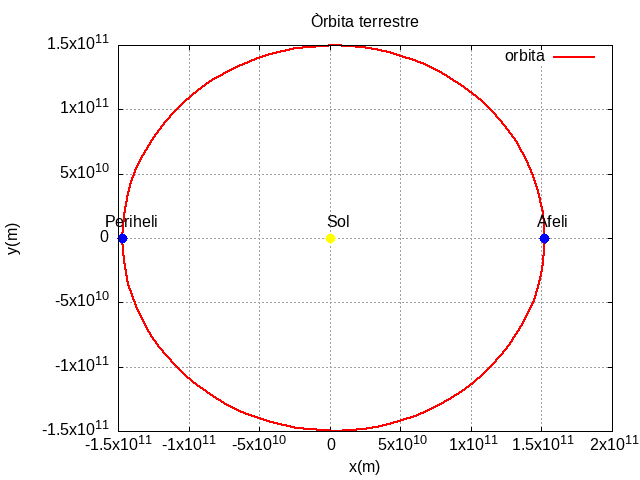
\includegraphics[width=0.5\textwidth]{orbita.png}
    \label{orb_terra}
    \caption{Òrbita Terrestre calculada numèricament}
\end{figure}

El mètode d'Euler és poc exacte però amb una discretització prou fina dona bons resultats. Si calculem l'error acomulat en el radi al completar una Òrbita sencera amb una discretització temporal de $3000$ punts obtenim
\begin{equation}
    Error = \frac{1.47098075136e11-1.47082017410e11}{1.47098075136e11}100\approx0,01\%
\end{equation}
Tot i així a la secció \ref{sec: edos} resoldrem aquest sistema d'EDOs amb altres mètodes per comparar-ne els resultats.


\section{Posició del Sol al cel vist des de l'habitatge} \label{sec: seccio_2}
En aquesta secció ens proposem trobar la posició del Sol des d'un punt determinat de la Terra durant tot l'any.\footnote{\label{nota: habitatge}Per fer els càlculs hem agafat les coordenades d'un habitatge de Sant Cugat del Vallès: 41°28'03.4"N 2°04'28.4"E} Per fer-ho hem parametritzat la posició del sol amb dos angles, l'angle vertical $\nu$ i l'angle horitzontal $\eta$ (\ref{fig: sist_sol}), i hem definit els vectors $\vec{\rho}$, del centre del Sol al punt de la superfície de la Terra, $\vec{r}$, del centre del Sol al punt de la superfície de la Terra, i $\vec{R}$, del centre del Sol al centre de la Terra (\ref{fig: sist_vectors}).
\begin{figure}[hbt]
    \centering
    \begin{subfigure}{0.5\textwidth}
        \centering
        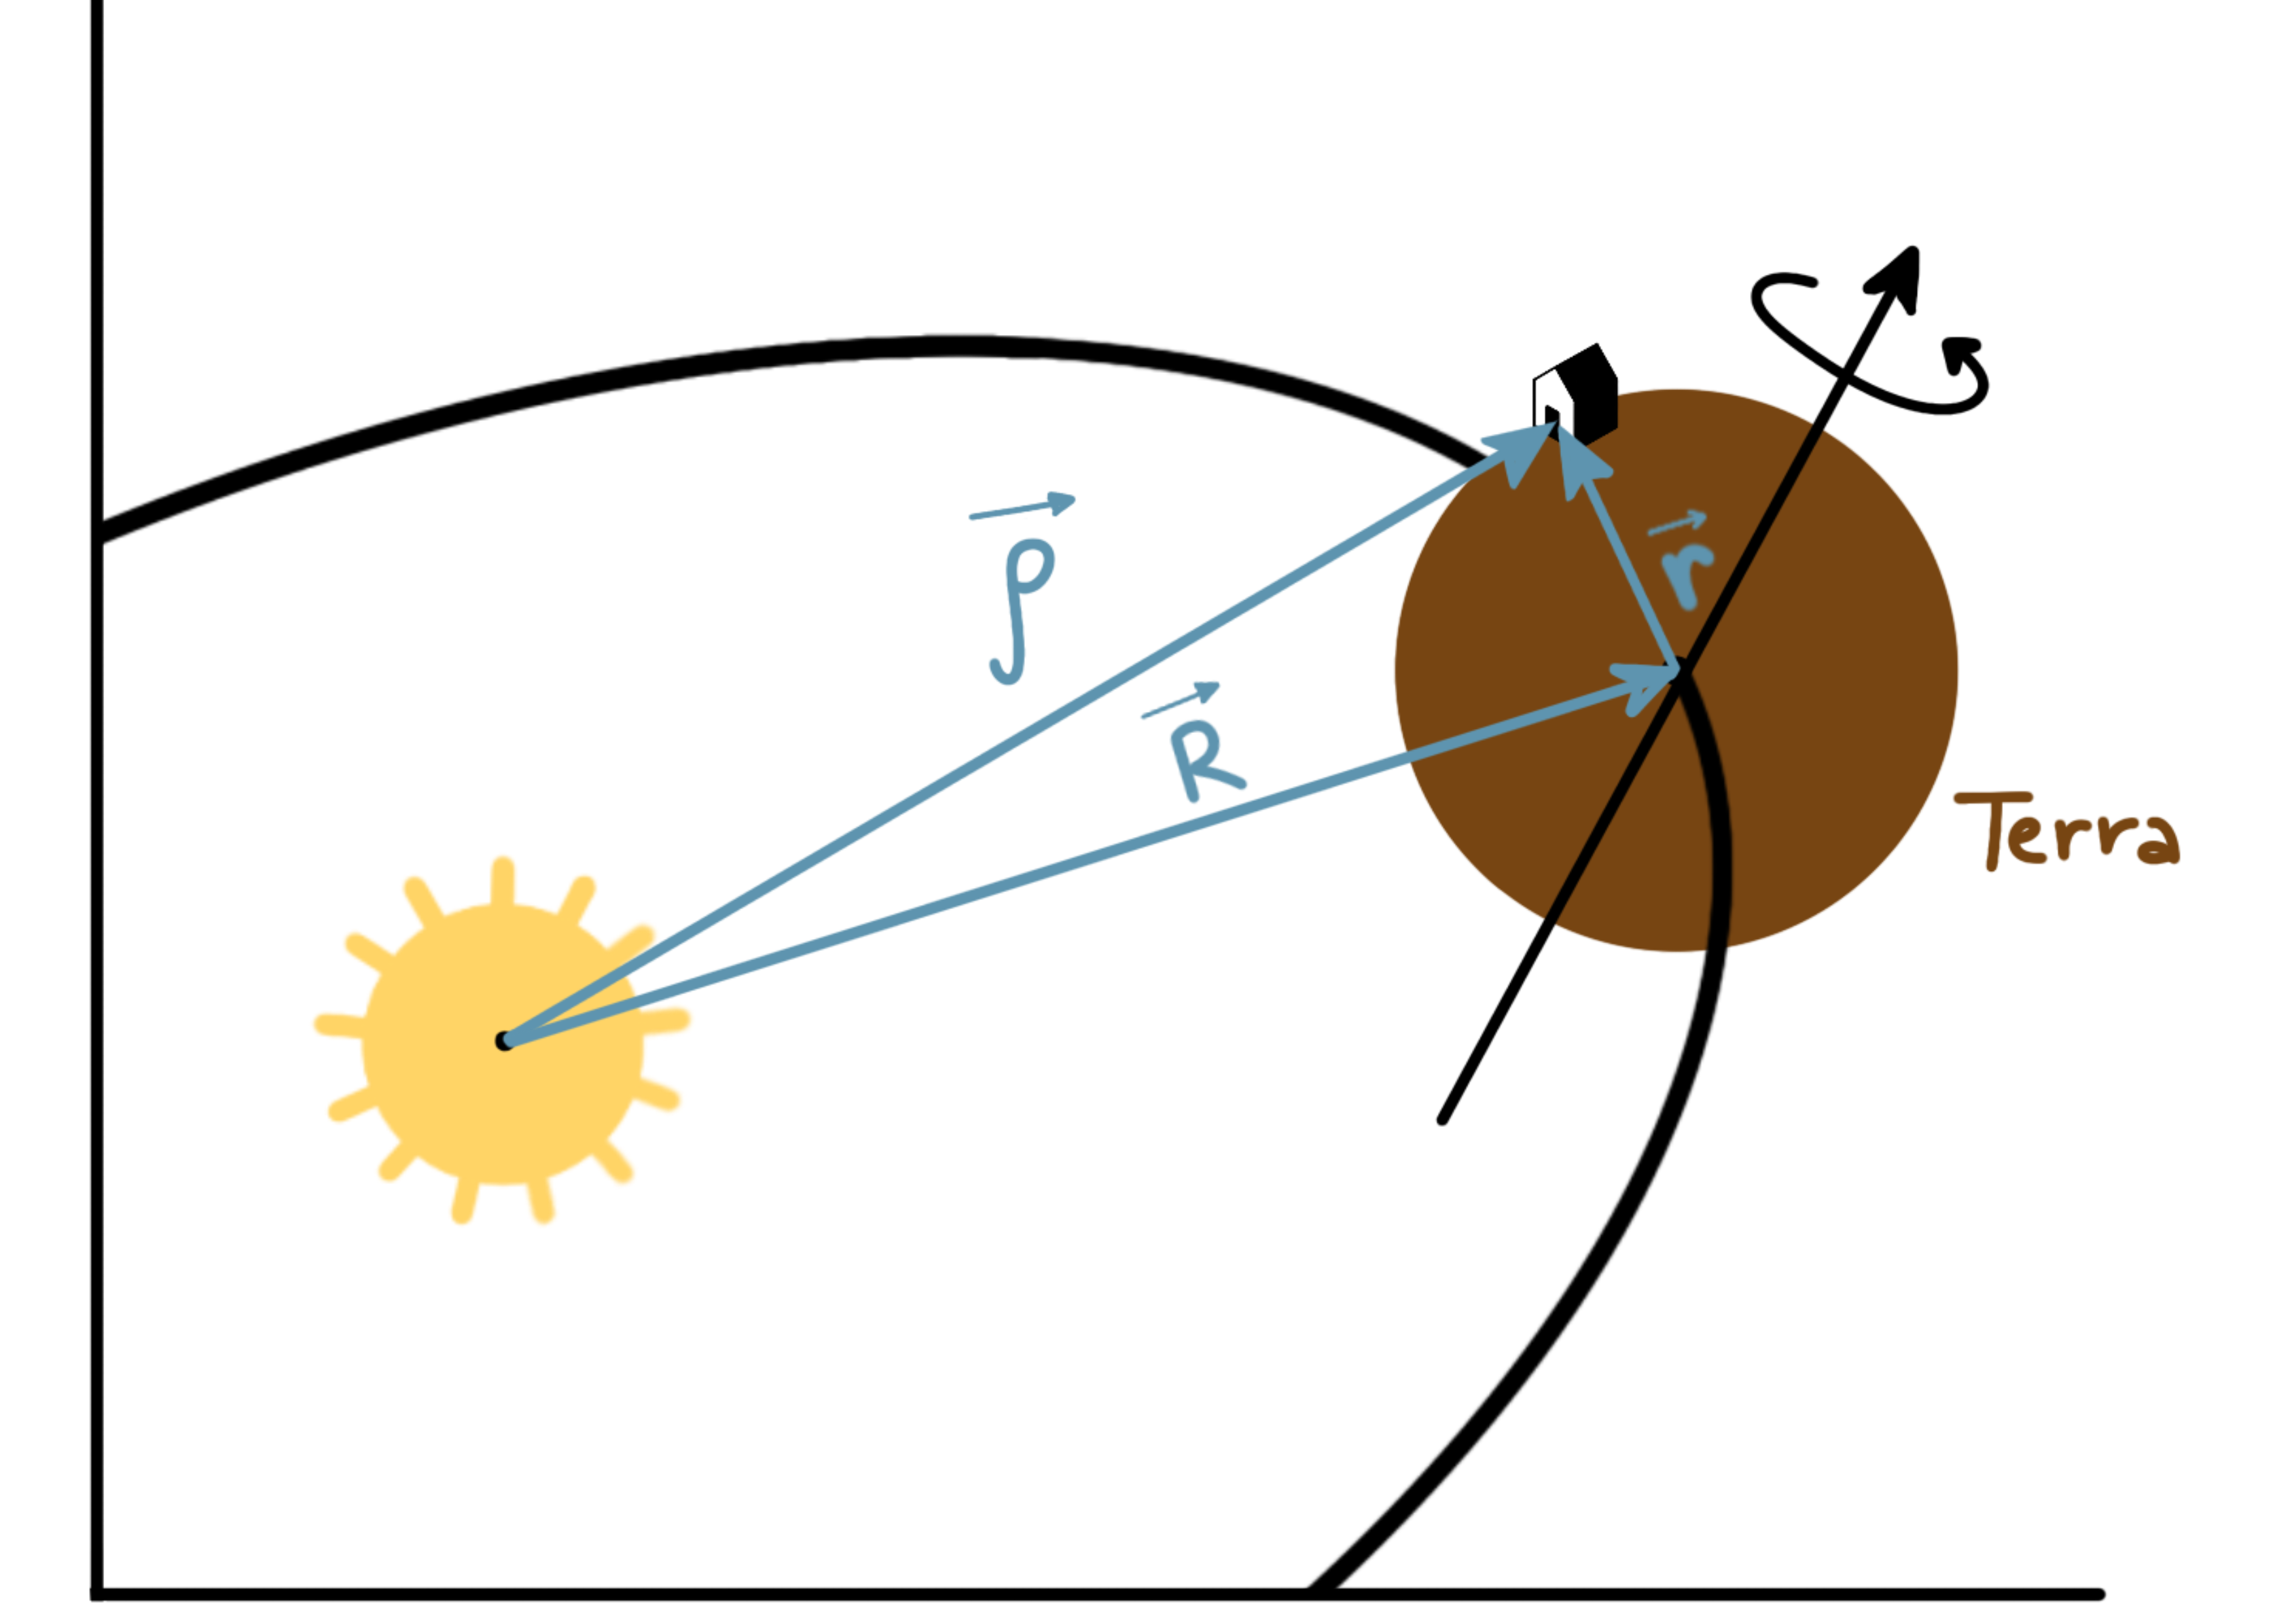
\includegraphics[width=\textwidth]{vectors.PNG}
        \caption{Els vectors que hem definit a la secció \ref{sec: seccio_2}.}
        \label{fig: sist_vectors}
    \end{subfigure}%
    \hspace{0.000001\textwidth}%
    \begin{subfigure}{0.5\textwidth}
        \centering
        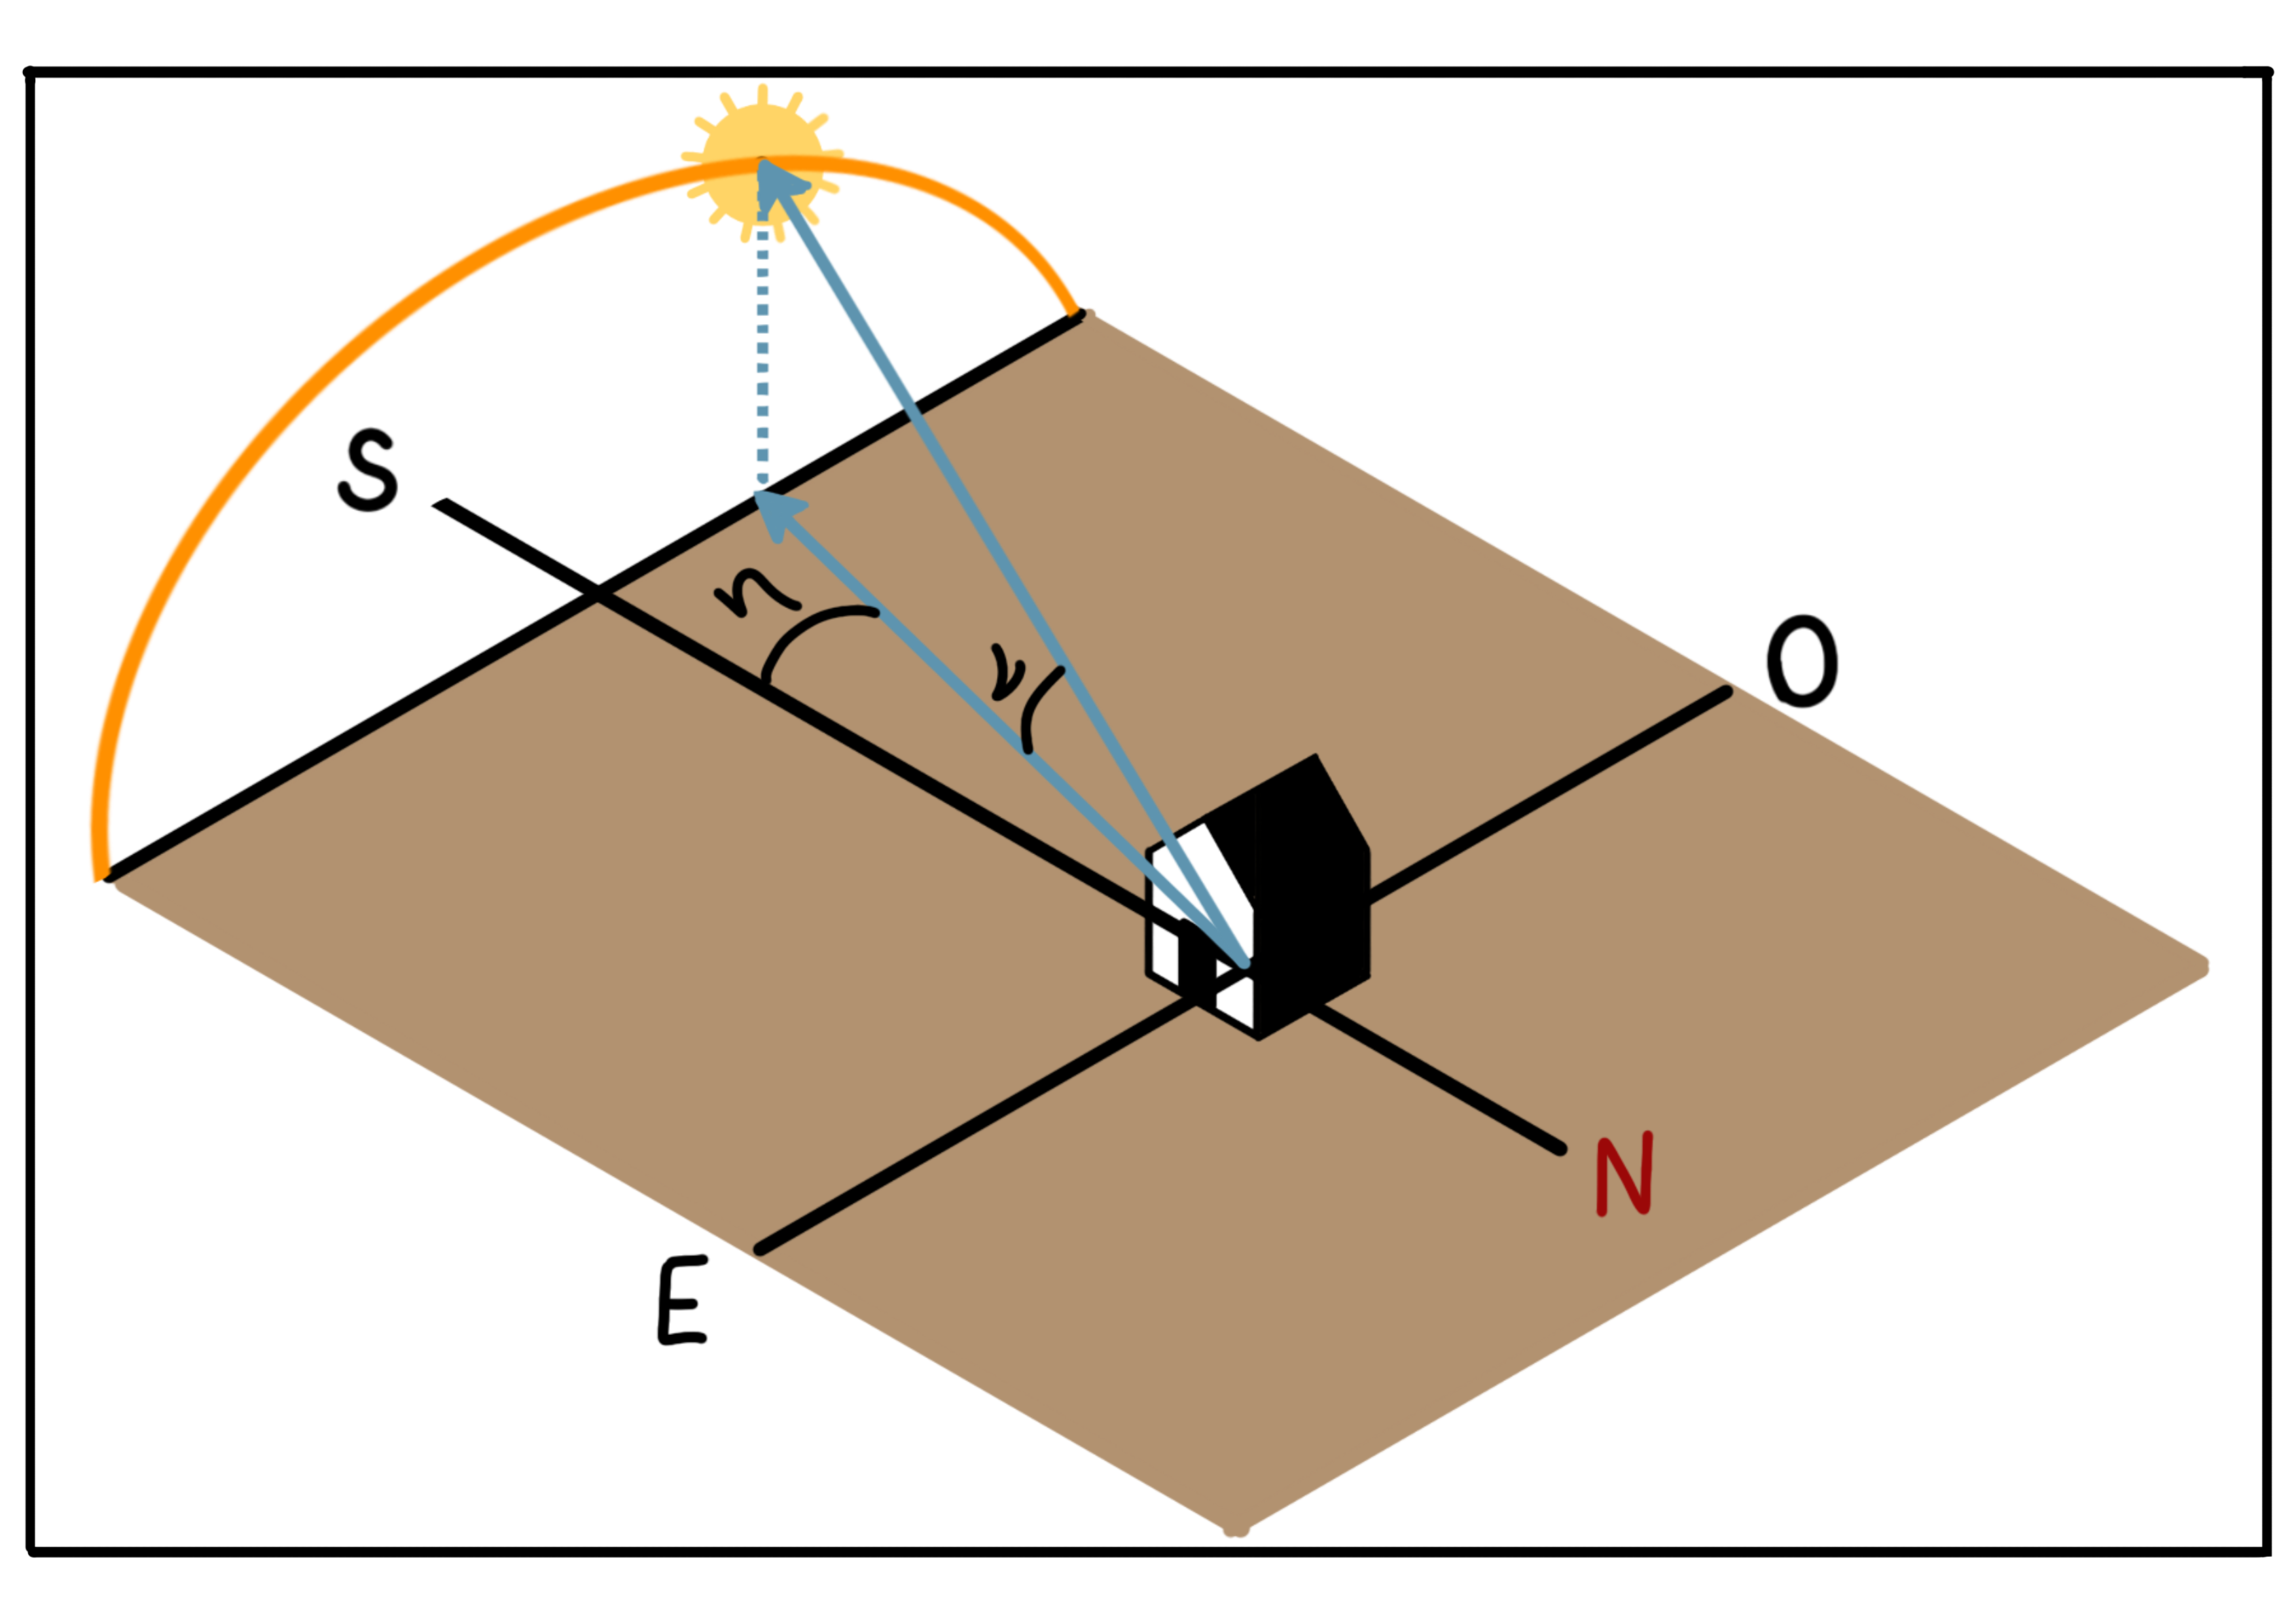
\includegraphics[width=\textwidth]{ang_sol.PNG}
        \caption{Els dos angles que hem usat per a determinar la posició del Sol.}
        \label{fig: sist_sol}
    \end{subfigure}
\end{figure}

També hem definit tres sistemes de referència (figura \ref{fig: sist_ref}) per facilitar els càlculs i trobar els àngles esmentats. Començant al sistema $\Omega$ podem obtenir un vector al sistema $\gamma$ a través de les matrius de rotació de l'annex \ref{annex: matr_rot}. Les relacions entre aquests sistemes són
\begin{itemize}
    \item Sistema $\Omega$: l'eix $z$ està orientat amb l'eix de rotació de la Terra.
    \item Sistema $\beta$: sistema rotat un angle $\beta$ en el pla $zy$ respecte el sistema $\Omega$. $\beta$ és l'angle entre l'eix de rotació de la terra i el vector perpendicular al pla de l'orbita, per tant, ara l'eix $z$ apunta en direcció pendicular al pla de l'òrbita.
    \item Sistema $\gamma$: sistema rotat un angle $\gamma$ en el pla $xy$ respecte el sistema $\beta$. $\gamma$ és l'angle entre $\vec{R}_{periheli}$ i $\vec{R}_{solstici(hivern)}$, per tant, ara la direcció de l'eix $y$ coincideix amb la direcció del periheli.
\end{itemize}
de tal manera que al sistema $\gamma$ tenim l'òrbita de la Terra amb el periheli i l'afeli sobre l'eix y i l'eix de rotació de la Terra orientat per tal que al solstici d'hivern (21 de Desembre) l'angle entre l'eix de rotació de la Terra i la direcció perpendicular al pla de l'òrbita sigui màxim.

Al sistema $\Omega$ el vector $\vec{r}$ és molt fàcil de definir 
\begin{equation}
    \vec{r}_{(t)}=r_T[\cos(\alpha)\cos(wt+\varphi)\hat{e_x}+\cos(\alpha)\sin(wt)+\varphi\hat{e_y}+\sin(\alpha)\hat{e_z}]
    \label{vector_r}
\end{equation}
si tenim la coordenada de latitud del punt de la Terra on volem fer els càlculs, $\alpha$, i el radi de la Terra, $r_T$, i on $w$ és la velocitat angular de rotació de la Terra i $t$ el temps transcorregut al llarg del dia.
Per tal de que aquest vector a $t=0$ comenci a la posició més allunyada del Sol (és a dir que t=0 es correspongui amb la meitat de la nit) hem d'afegir l'angle $\varphi$ a l'angle de rotació. $\varphi$ anirà variant cada dia i és l'angle entre el vector definit a (\ref{vector_r}) i el vector $\vec{R}$ a $t=0$.

El vector $\vec{R}$ ja el tenim calculat de la secció \ref{sec: seccio_1} i el vector $\vec{\rho}$ és simplement
\begin{equation}
    \vec{\rho}= \vec{R}+\vec{r}
\end{equation}
Un cop tenim aquests tres vectors els angles queden definits
\begin{equation}
    \nu=\angle (\vec{r}_{\gamma}, \vec{\rho}_{\gamma}) -\frac{\pi}{2}  
\end{equation}
\begin{equation}
    \eta=\pi - \angle (\vec{R}_{\Omega}, \vec{r}_{\Omega})
\end{equation}
on usem la funció arccosinus per trobar els angles.\footnote{$\angle (\vec{u}, \vec{v})= \arccos\left(\frac{\vec{u} \cdot \vec{v}}{\|\vec{u}\| \|\vec{v}\|}\right)$}


Si calculem aquests angles per una posició concreta a la Terra\footref{nota: habitatge}i pels dies que corresponen als equinocis i als solsticis obtenim el següent gràfic.
\begin{figure}[H]
    \centering
    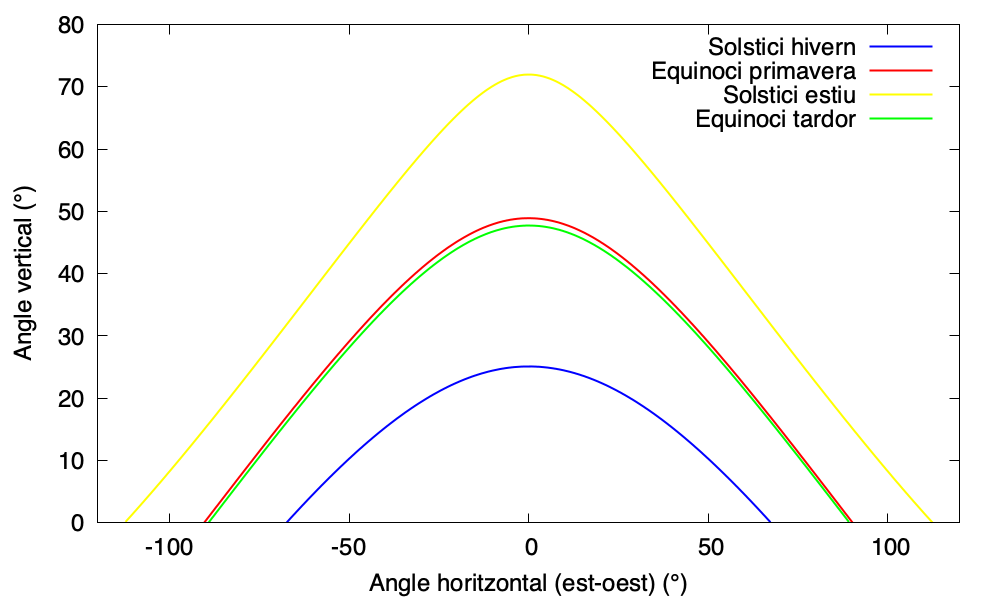
\includegraphics[width=0.5\textwidth]{equinocis.png}
    \label{solsticis}
    \caption{Angles del Sol al llarg d'un dia per diferents moments de l'any a un habitatge de Sant Cugat del Vallès}
\end{figure}

\section{Estudi energètic de la placa}
\subsection{Potència elèctrica produïda per un panell solar}
Suposant que el Sol és un cos negre esfèric a temperatura $T_S$ i de radi $R_S$, utilitzant la llei de Stefan-Boltzmann la potència que emet és $P_S=\sigma_{SB}T_S^44\pi R_S^2$. La intensitat de la radiació en un punt a una distància ${\rho}$ del Sol $I_{\rho}$ és igual la potència $P_S$ dividida entre l'àrea del front d'ona de la radiació, que és una closca esfèrica de radi ${\rho}$. Si el punt es troba a la superfície terrestre,  per l’efecte de l’albedo $\alpha_A$ cal multiplicar $I_{\rho}$ per $\alpha=1-\alpha_A$, la fracció de radiació absorbida per la Terra. Així doncs, la intensitat de la radiació incident és:
\begin{equation}
    I_{abs} = \frac{P_S}{4\pi d^2}=\frac{1}{d^2}R_S^2\sigma_SB T_S^4 \ .
    \label{I_abs}
\end{equation}
La intensitat efectiva que rebrà un panell solar és $I_{abs} \cos{\theta}$, on $\theta$ és l'angle entre la direcció de la llum incident i la normal al panell. Finalment, la potència elèctrica generada és igual al producte d'aquesta intensitat multiplicada per l'àrea del panell, $A$, i per un factor $r$, el seu rendiment. Aleshores,
\begin{equation}
    P = r I_{abs} A \cos{\theta} = r \alpha \frac{1}{\rho^2}R_S^2\sigma_{SB}T_S^4A \cos{\theta} \ .
    \label{potencia placa}
\end{equation}
Els valors numèrics de $\alpha$, $R_S$, $\sigma_{SB}$ i $T_S$ els hem obtingut de les fonts \cite{Earth Fact Sheet}, \cite{Sun Fact Sheet} i \cite{Universe Glossary}.

A continuació normalitzem aquesta expressió. En quant a la variable $\theta$, al tractar-se d'un angle ja és adimensional, i per tant la donem per normalitzada. En quant a les altres dues variables,
\begin{align}
    \hat{P}=\frac{P}{400} \label{P normalizada} \\
    \hat{\rho}= \rho \left( r \alpha R_S^2\sigma_{SB}T_S^4A/400 \right)^{-1/2} \label{rho normalizada}
\end{align}
on hem escollit el valor 400 W per a normalitzar la potència. Segons l'enunciat, és la màxima electricitat $P_{max}$ que pot generar la placa per $I=10^3$ W/$\text{m}^2$ de radiació incident. També utilitzem aquests valors per trobar el valor del rendiment $r$ de la placa de la següent manera:
\begin{equation}
     r = \frac{P_{max}}{IA} \ .
\end{equation}
Així doncs, segons aquesta normalització l'Eq. \eqref{potencia placa} esdevé:
\begin{equation}
    \hat{P} = \frac{\cos{\theta}}{\hat{\rho}^2} \ .
    \label{pot norm}
\end{equation}
Per a determinar $\cos{\theta}$, utilitzem la següent expressió:
\begin{equation}
    \cos \theta = \cos \theta_z \cos \beta + \sin \theta_z \sin \beta \cos (\eta - \gamma) \ .
    \label{cos theta}
\end{equation}
amb $\theta_z = 90^{\circ}-\nu$, on els angles $\eta$ i $\nu$ ja han estat definits i calculats a la secció anterior, i són les variables que determinen $\theta$. Els angles $\beta$ i $\gamma$ són paràmetres que fan referència a la inclinació i orientació de la placa; es defineixen formalment a la secció \ref{sec: demo cos theta} de l'Annex, on es demostra l'equació.

A la Figura següent es representa la potència en funció del temps en dos dies diferents.

\begin{figure}[H]
    \centering
    \begin{subfigure}{0.5\textwidth}
        \centering
        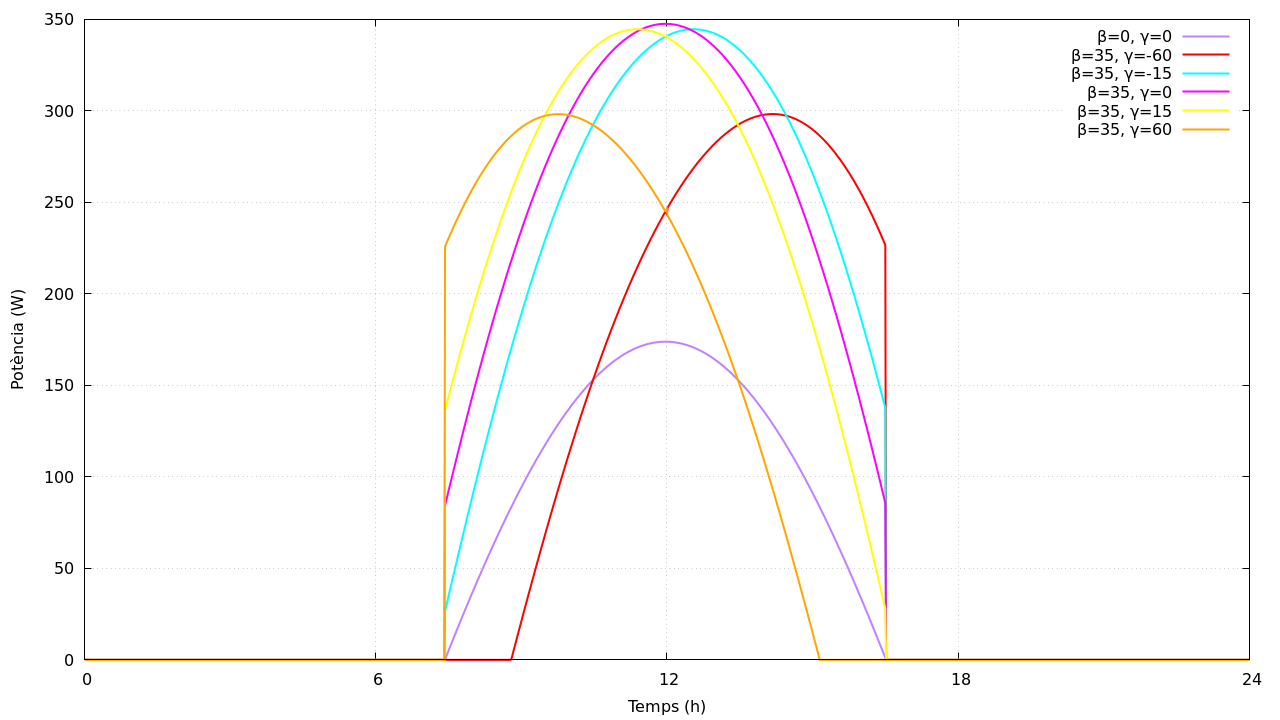
\includegraphics[width=\textwidth]{dia1_pot_plot.png}
        \caption{Potència elèctrica produïda per la placa durant un dia.}
        \label{fig: potencia}
    \end{subfigure}%
    \hspace{0.000001\textwidth}%
    \begin{subfigure}{0.5\textwidth}
        \centering
        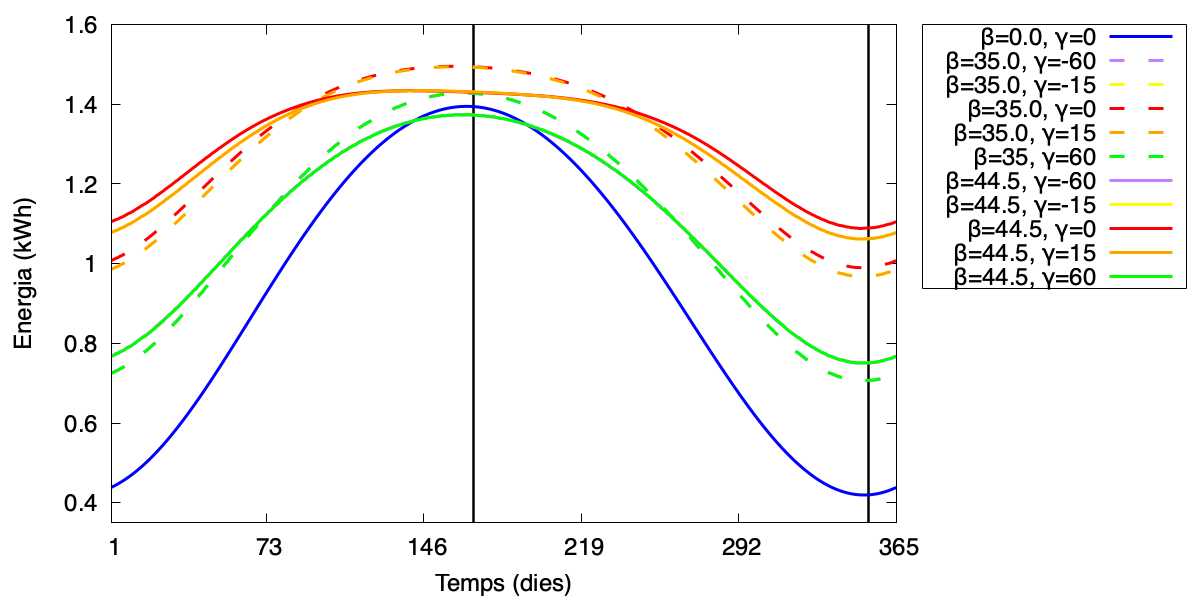
\includegraphics[width=\textwidth]{energia.png}
        \caption{Energia elèctrica produïda per la placa cada dia de l'any.}
        \label{fig: energia}
    \end{subfigure}
    \caption{Gràfics referents a l'estudi energètic de la placa.}
    \label{estudi energia}
\end{figure}

Quan $\beta=0^{\circ}$, es representa la gràfica per un sol valor de $\gamma$ (escollim arbitràriament $\gamma=0^{\circ}$) perquè el terme $\sin\beta$ en l’Eq. \eqref{cos theta} s’anul·la i, per tant, desapareix la dependència en $\gamma$.

Si $\theta_z$ o $\theta$ surten del rang $[-\pi/2,\pi/2]$ hem imposat que la potència sigui nul·la. Quan $\theta \notin [-\pi/2,\pi/2]$, el Sol es troba per sota de l'horitzó, impedint que arribi llum a la placa. És per això que mentre que per $\beta = 0^{\circ}$ la potència s'anul·la gradualment, per $\beta \neq 0^{\circ}$ s'anul·la bruscament, ja que quan el Sol és a prop de l’horitzó $\theta$ encara és inferior a $90^{\circ}$. Similarment, quan $\theta \notin [-\pi/2,\pi/2]$ el Sol està situat darrere la placa, sent ella mateixa la que bloqueja la llum. És per això que quan $\gamma$ és prou gran, com ara en la Fig. \ref{fig: potencia dia 1} per $\gamma=\pm60^{\circ}$, la potència s'anul·la abans que el Sol estigui a l'horitzó.

\subsection{Energia elèctrica produïda per un panell solar}
Amb la potència elèctrica generada per la placa cada minut de l'any ens disposem a calcular l'energia elèctrica produïda per aquesta. La potència és la derivada temporal de l'energia, per tant, podem trobar l'energia elèctrica produïda per la placa durant una certa quantitat de temps integrant numèricament la potència respecte el temps. Per fer-ho, hem optat pel mètode d'integració numèrica de Simpson $\frac{1}{3}$. Presentem l'energia produïda cada dia de l'any per diferents combinacions dels angles $\beta$ (inclinació i orientació de la placa) i $\gamma$ (orientació de la placa) a la Fig. \ref{fig: energia}.


%\begin{figure}[H]
    %\centering
    %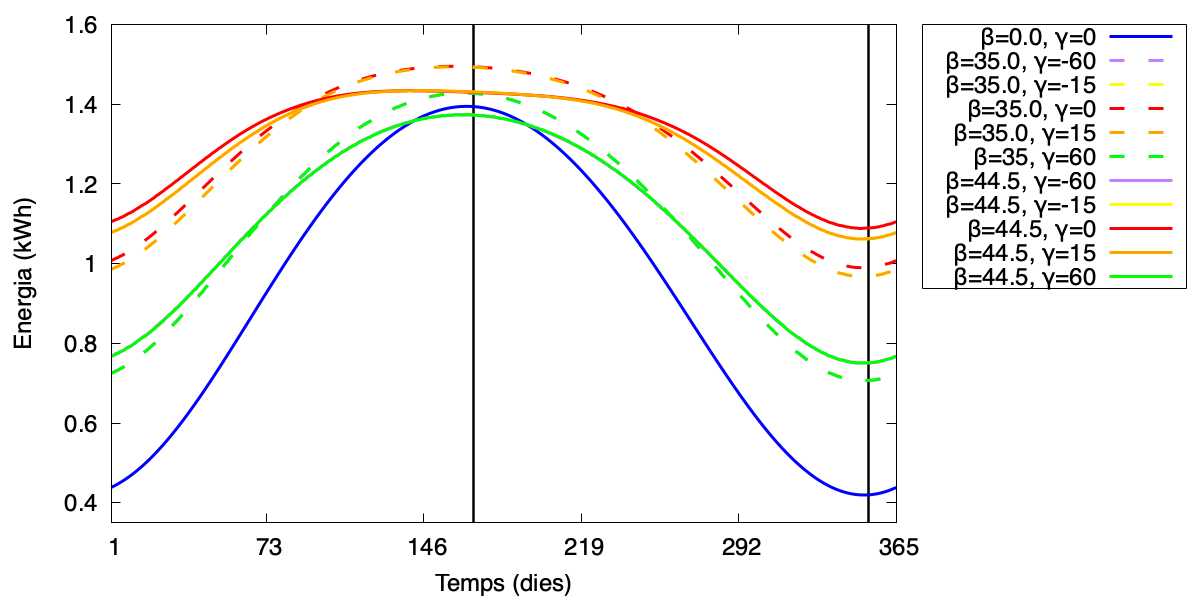
\includegraphics[width=0.75\linewidth]{energia.png}
    %\caption{Energia elèctrica produïda per la placa cada dia de l'any.}
    %\label{fig: energies}
%\end{figure}

Les linies negres verticals indiquen els solsticis d'estiu i d'hivern per a una millor interpretació dels resultats.

Pel que fa a la normalització del problema numèric, ens ha quedat la següent equació normalitzada.
\begin{equation}
    \hat{E} = \int \hat{P} \, d\hat{t}
    \label{energia}
\end{equation}
on $\hat{t}=\frac{t}{t_0}$, $\hat{P}=\frac{P}{P_0}$ i $\hat{E}=\frac{E}{P_0 t_0}$, amb $t_0=86400$ s (els segons que hi ha en un dia) i $P_0=400$ W (la potència màxima de la placa en les condicions donades a l'enunciat de la pràctica). 
\subsection{Extra: Optimització dels angles de la placa}

Hem plantejat el problema des del punt de vista de maximitzar la producció d'energia total al llarg d'un any mantenint els angles $\beta$ i $\gamma$ de la placa constants durant tot l'any. Per fer-ho, hem utilitzat que si tenim en compte l'Eq. \ref{potencia placa} i \ref{cos theta}, l'energia total normalitzada produïda en un any la podem escriure com
\[
\hat{E}_T(\beta, \gamma) = \cos \beta \int \hat{P}_{opt} \cos \theta_{z} \, d\hat{t} + \sin \beta \cos \gamma \int \hat{P}_{opt} \sin \theta_{z} \cos \eta \, d\hat{t} + \sin \beta \sin \gamma \int \hat{P}_{opt} \sin \theta_{z} \sin \eta \, d\hat{t} \equiv
\]
\[
\equiv \hat{a}\cos \beta
+ \hat{b}\sin \beta \cos \gamma
+ \hat{c}\sin \beta \sin \gamma
\]
on $\hat{P}_{opt}=\frac{r I_{abs} A}{P_0}$, $\hat{t}=\frac{t}{t_0}$ i $\hat{E}=E P_0 t_0$

Igualant el gradent a 0, trobem que
\[
\left.
\begin{aligned}
-\hat{a}\sin \beta + \hat{b}\cos \beta \cos \gamma + \hat{c}\cos \beta \sin \gamma = 0 \\
-\hat{b}\sin \beta \sin \gamma + \hat{a}\sin \beta \cos \gamma = 0
\end{aligned}
\right\}
\]
La solució corresponent per $\beta$ i $\gamma$ és
\[
\gamma = \arctan\left(\frac{\hat{c}}{\hat{b}}\right), \quad \beta = \arctan\left(\frac{\hat{b} \cos(\gamma) + \hat{c} \sin(\gamma)}{\hat{a}}\right)
\]
on hem descartat la solució corresponent a $\beta=n\pi$ per no ser un màxim.

Calculant numèricament les integrals $\hat{a}$, $\hat{b}$ i $\hat{c}$ per Simpson 1/3 sota la condició de que $-\frac{\pi}{2} \leq \theta_z \leq \frac{\pi}{2}$ (en cas contrari l'integrand l'hem anul·lat), hem obtingut uns angles òptims arrodonint a la primera xifra decimal de $\gamma=0^\circ$ i $\beta=44,5^\circ$. L'energia produïda dia a dia durant tot l'any corresponent a aquests angles pot trobar-se a la Fig. \ref{fig: energia}. 

A la Fig. \ref{fig: energies} podem observar que a l'estiu un angle d'inclinació de $35^\circ$, per exemple, produeix més energia que un de $44,5^\circ$, ara bé, com hem dit, nosaltres hem maximitzat la producció total durant l'any. Això, però, suggereix que durant diferents èpoques de l'any podriem modificar la inclinació de la placa per així maximitzar la seva producció en cada període i conseqüentment durant tot l'any.

\section{Resolució de l'EDO per diversos mètodes numèrics}\label{sec: edos}
Per a resoldre l'EDO de l'òrbita terrestre hem utilitzat el mètode d'Euler, però sabem que hi ha mètodes numèrics més potents que aquest. Per axò hem volgut comparar els resultats.

Els mètodes emprats per a resoldre l'equació \eqref{equ_en_r} han estat el Runge-Kutta d'ordre 2 i el Runge-Kutta d'ordre 4, amb la mateixa discretització temporal en els 3 mètodes numèrics.

\begin{figure}[H]
    \centering
    \begin{subfigure}{0.5\textwidth}
        \centering
        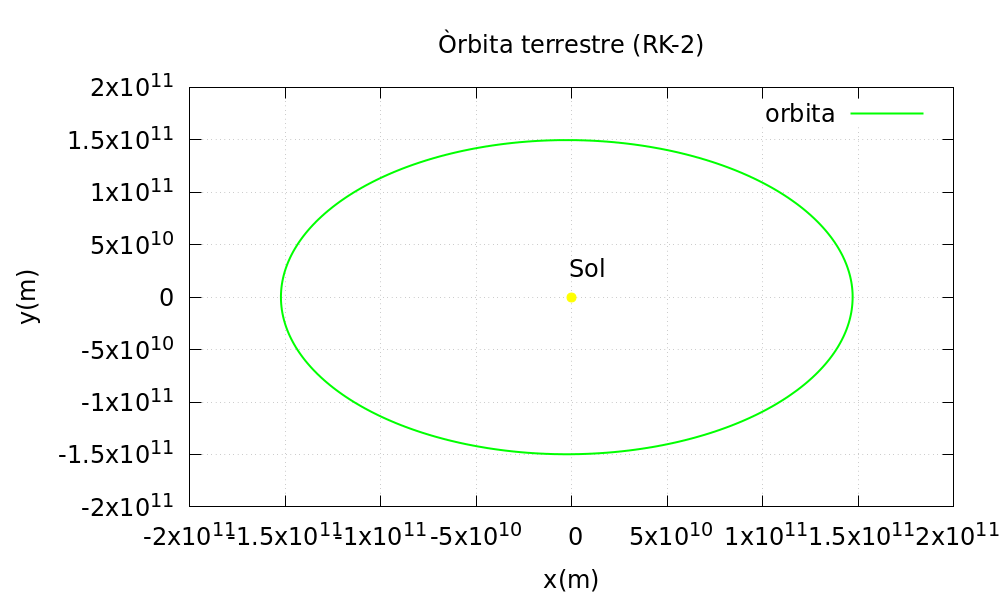
\includegraphics[width=\textwidth]{orbitaRK2.PNG}
        \caption{Òrbita terrestre per Runge-Kutta d'ordre 2}
        \label{fig: orbitaRK2}
    \end{subfigure}%
    \vspace{0.01\textwidth}%
    \begin{subfigure}{0.5\textwidth}
        \centering
        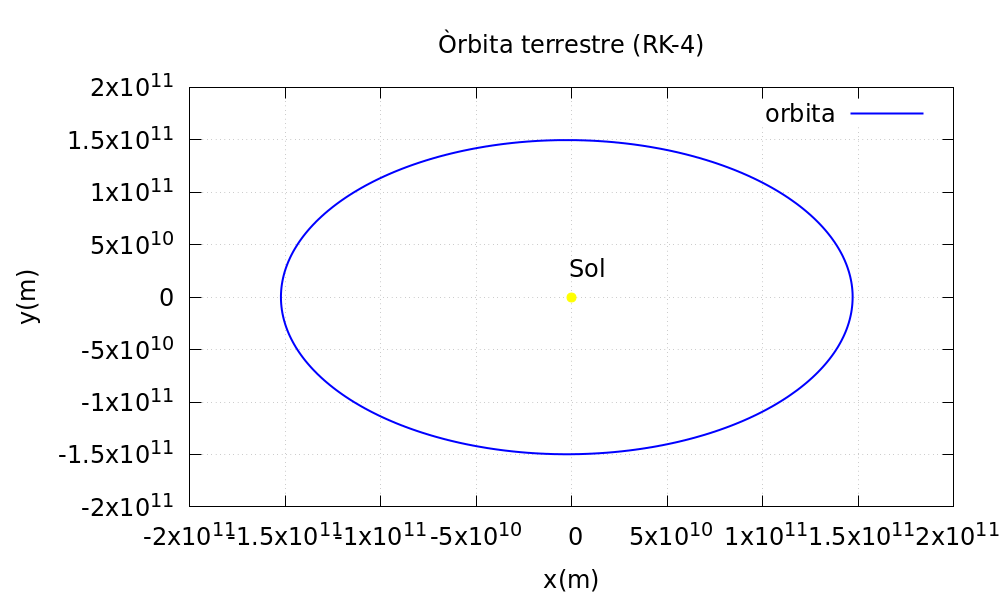
\includegraphics[width=\textwidth]{orbitaRK4.PNG}
        \caption{Òrbita terrestre per Runge-Kutta d'ordre 4}
        \label{fig: orbitaRK4}
    \end{subfigure}
    \vspace{0.01\textwidth}%
    \begin{subfigure}{0.5\textwidth}
        \centering
        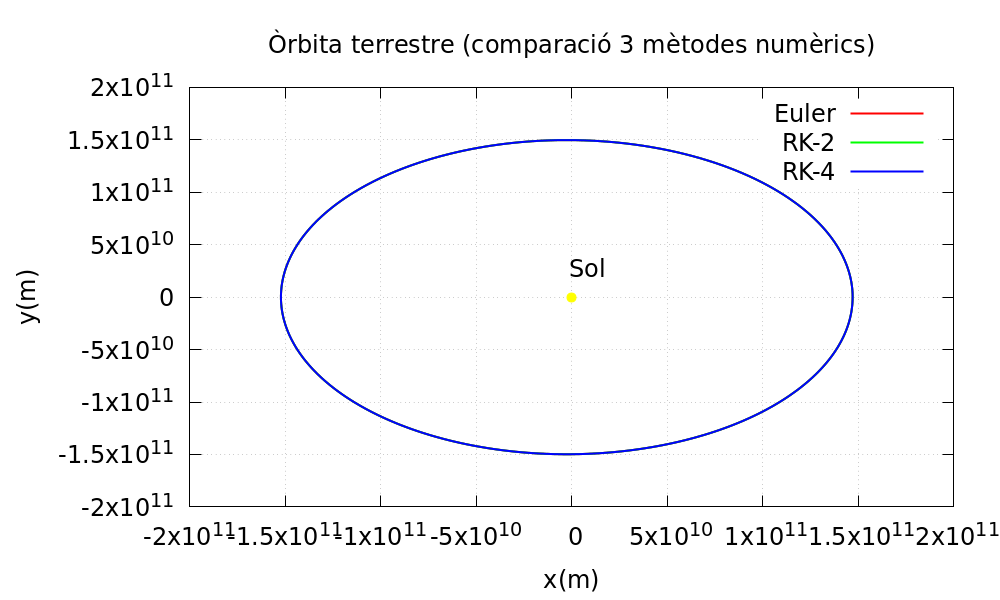
\includegraphics[width=\textwidth]{orbita3met.PNG}
        \caption{Òrbites terrestres per 3 mètodes numèrics}
        \label{fig: orbita3met}
    \end{subfigure}
    \caption{Càlcul òrbita terrestre per diferents mètodes numèrics}
    \label{fig: grafics3met}
\end{figure}

Observant els gràfics \ref{fig: grafics3met} podem veure que les diferències entre les òrbites càlculades pels diferents mètodes numèrics són realment mínimes.

\section{Consideració de la Terra com no esfèrica}\label{sec: terranoesfera}
Fins ara hem estat considerant que la Terra tenia forma d'una esfera perfecta. Però sabem que realment, la força centrífuga generada per la seva pròpia rotació provoca una deformació en els pols, "aixafant-la" i fent que la Terra no sigui una esfera.

Això no ens afecta al càlcul de l'òrbita terrestre ja que aquesta només considera la distància del sol al centre de la Terra però sí afecta en la resta de càlculs ja que el Radi de la Terra deixa de ser constant. En aquest apartat, aproximarem la Terra a un esferoide, com a un el·lipsoide de revolució\footnote{\label{nota: elipsoide}Els semieixos que hem agafat per a calcular el radi de la terra com a una esferoide són a = 6378136.6 i b = 6356751.9, extrets de l'article de Viquikipèdia: El·lipsoide de referència}

\begin{figure}[H]
    \centering
    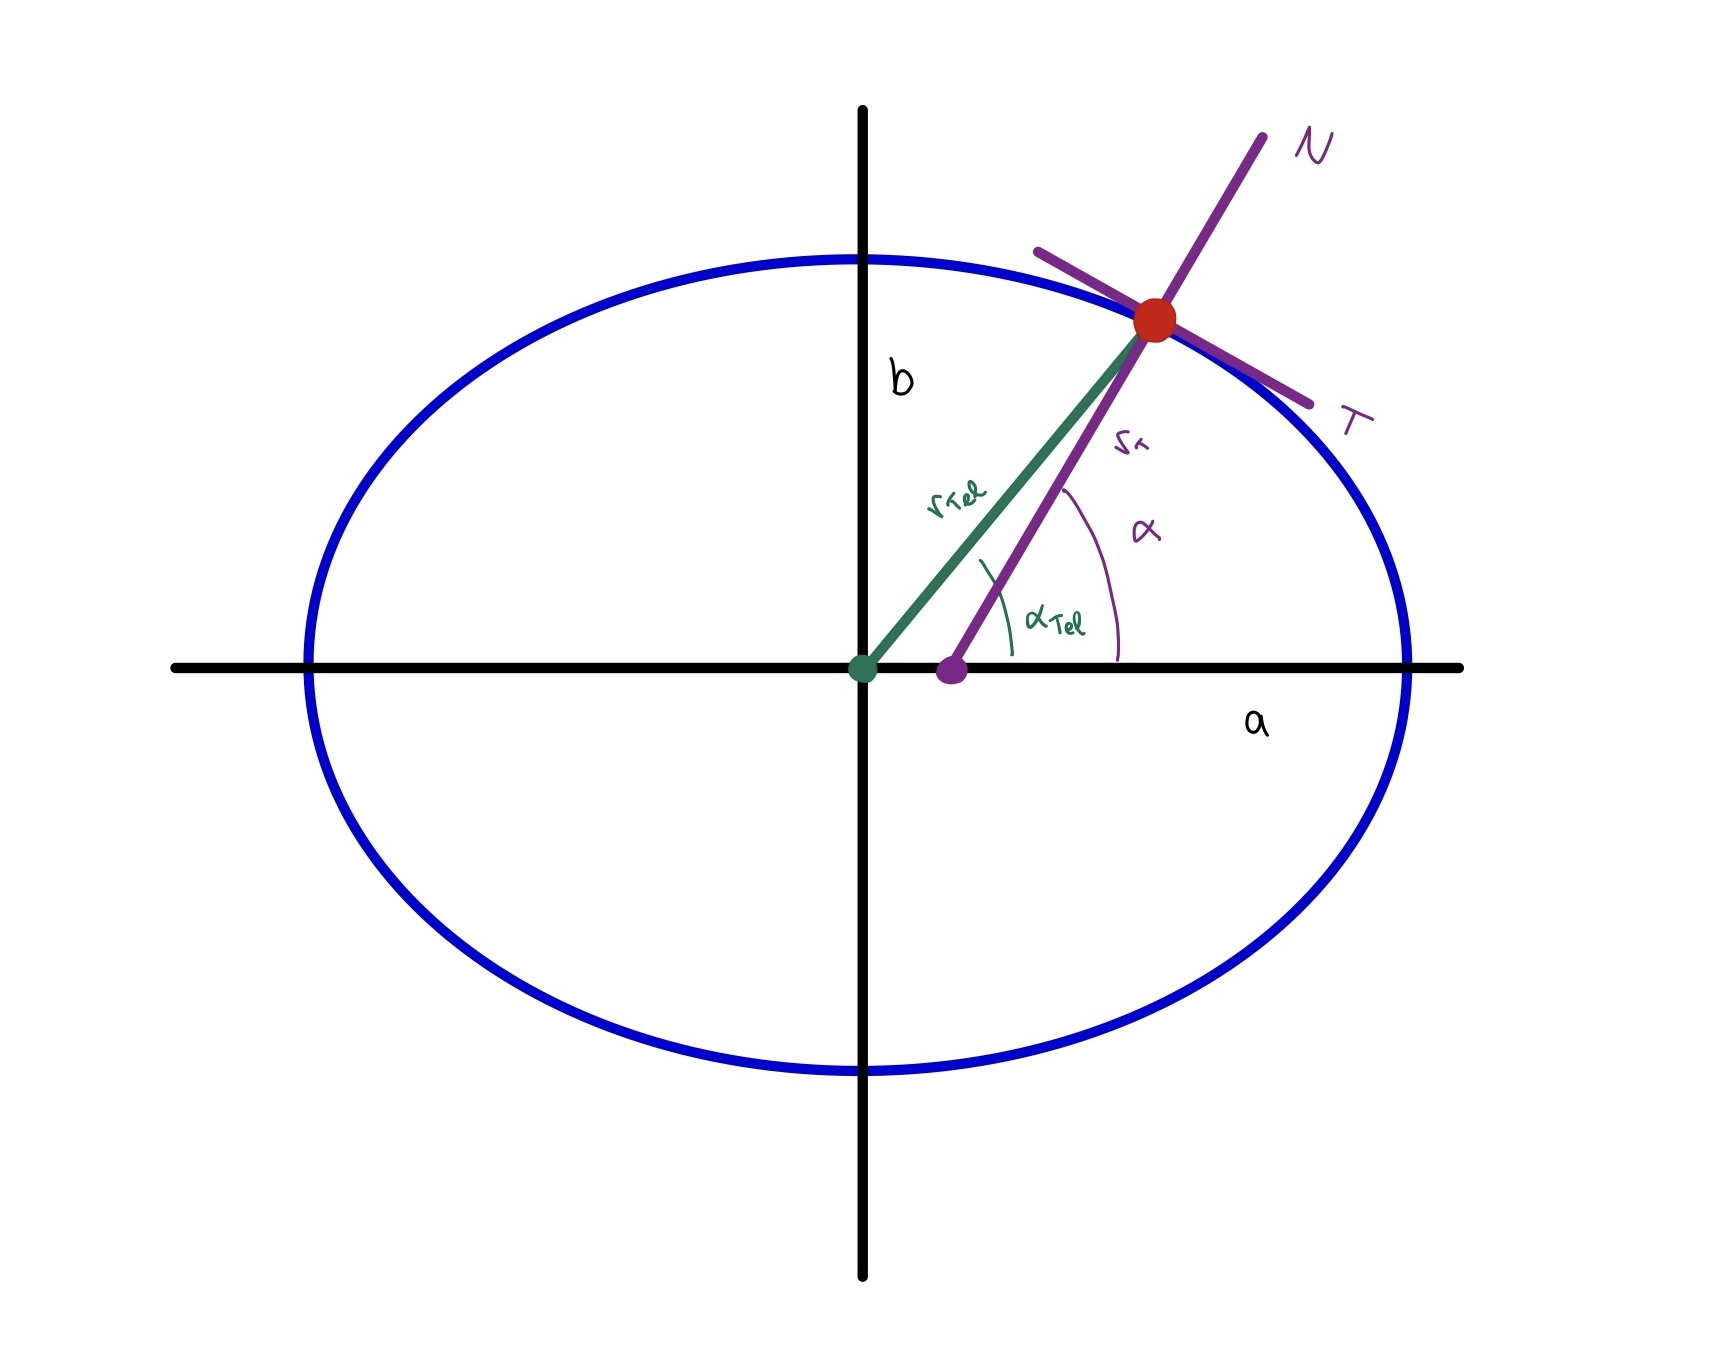
\includegraphics[width=0.5\textwidth]{Terraelipsoide.jpg}
    \caption{Aproximació de la Terra a un el·lipsoide de revolució, amb els angles i semieixos que hem d'utilitzat per recalcular el Radi Terrestre i l'angle de Latitud}
    \label{fig:terraelipsoide}
\end{figure}

Observant la figura \ref{fig:terraelipsoide}, podem acabar arribant a les següents expressions:

\begin{equation}
    tan(\alpha_{T_{el}}) = \frac{b}{a}tan(\alpha) 
\end{equation}

\begin{equation}
    r_{T_{el}} = \sqrt{\frac{(a^2cos(\alpha))^2+(b^2sin(\alpha))^2}{(acos(\alpha))^2+(bsom(\alpha))^2}}
\end{equation}

Aquesta ens permet calcular el Radi de la nostra esferoide (distància superfície-centre terreste) en funció de l'angle de latitud $\alpha$, calculat ja a partir de la dades geogràfiques en la secció \ref{sec: seccio_2}. Redefinim $r_T$ com $r_{T_el}$ i $\alpha$ com $\alpha_{T_{el}}$ per poder calcular el nou vector $\vec{r_{(t)}}$ amb l'equació \eqref{dist_centresup}. Els passos per a la simulació són exactament els mateixos que els ja definits a les corresponents seccions \ref{sec: seccio_2} i \ref{sec: seccio_3}.

\section*{Annex}
\appendix

\section{Link al repositori}
\vspace{-1em}
A continuació donem el link per a accedir al repositori de github on es troba el codi: \href{https://github.com/isaacbg25/Sol/tree/main}{link}

\section{Matrius de canvi de sistema de referència}\label{annex: matr_rot}
\begin{equation}
    \mathbf{R}_{\beta}=
    \begin{pmatrix}
      1 & 0 & 0   \\
      0 & \cos\beta& -sin\beta \\
      0 & sin\beta & cos\beta \\
    \end{pmatrix}
\end{equation}  

\begin{equation}
    \mathbf{R}_{\gamma}=
    \begin{pmatrix}
       \cos\beta& -sin\beta& 0 \\
       \sin\beta & cos\beta &0\\
      0 & 0 & 1  \\
    \end{pmatrix}
\end{equation}  


\section{Angles i vectors apartat 2}
\begin{figure}[hbt]
    \centering
    \begin{subfigure}{0.5\textwidth}
        \centering
        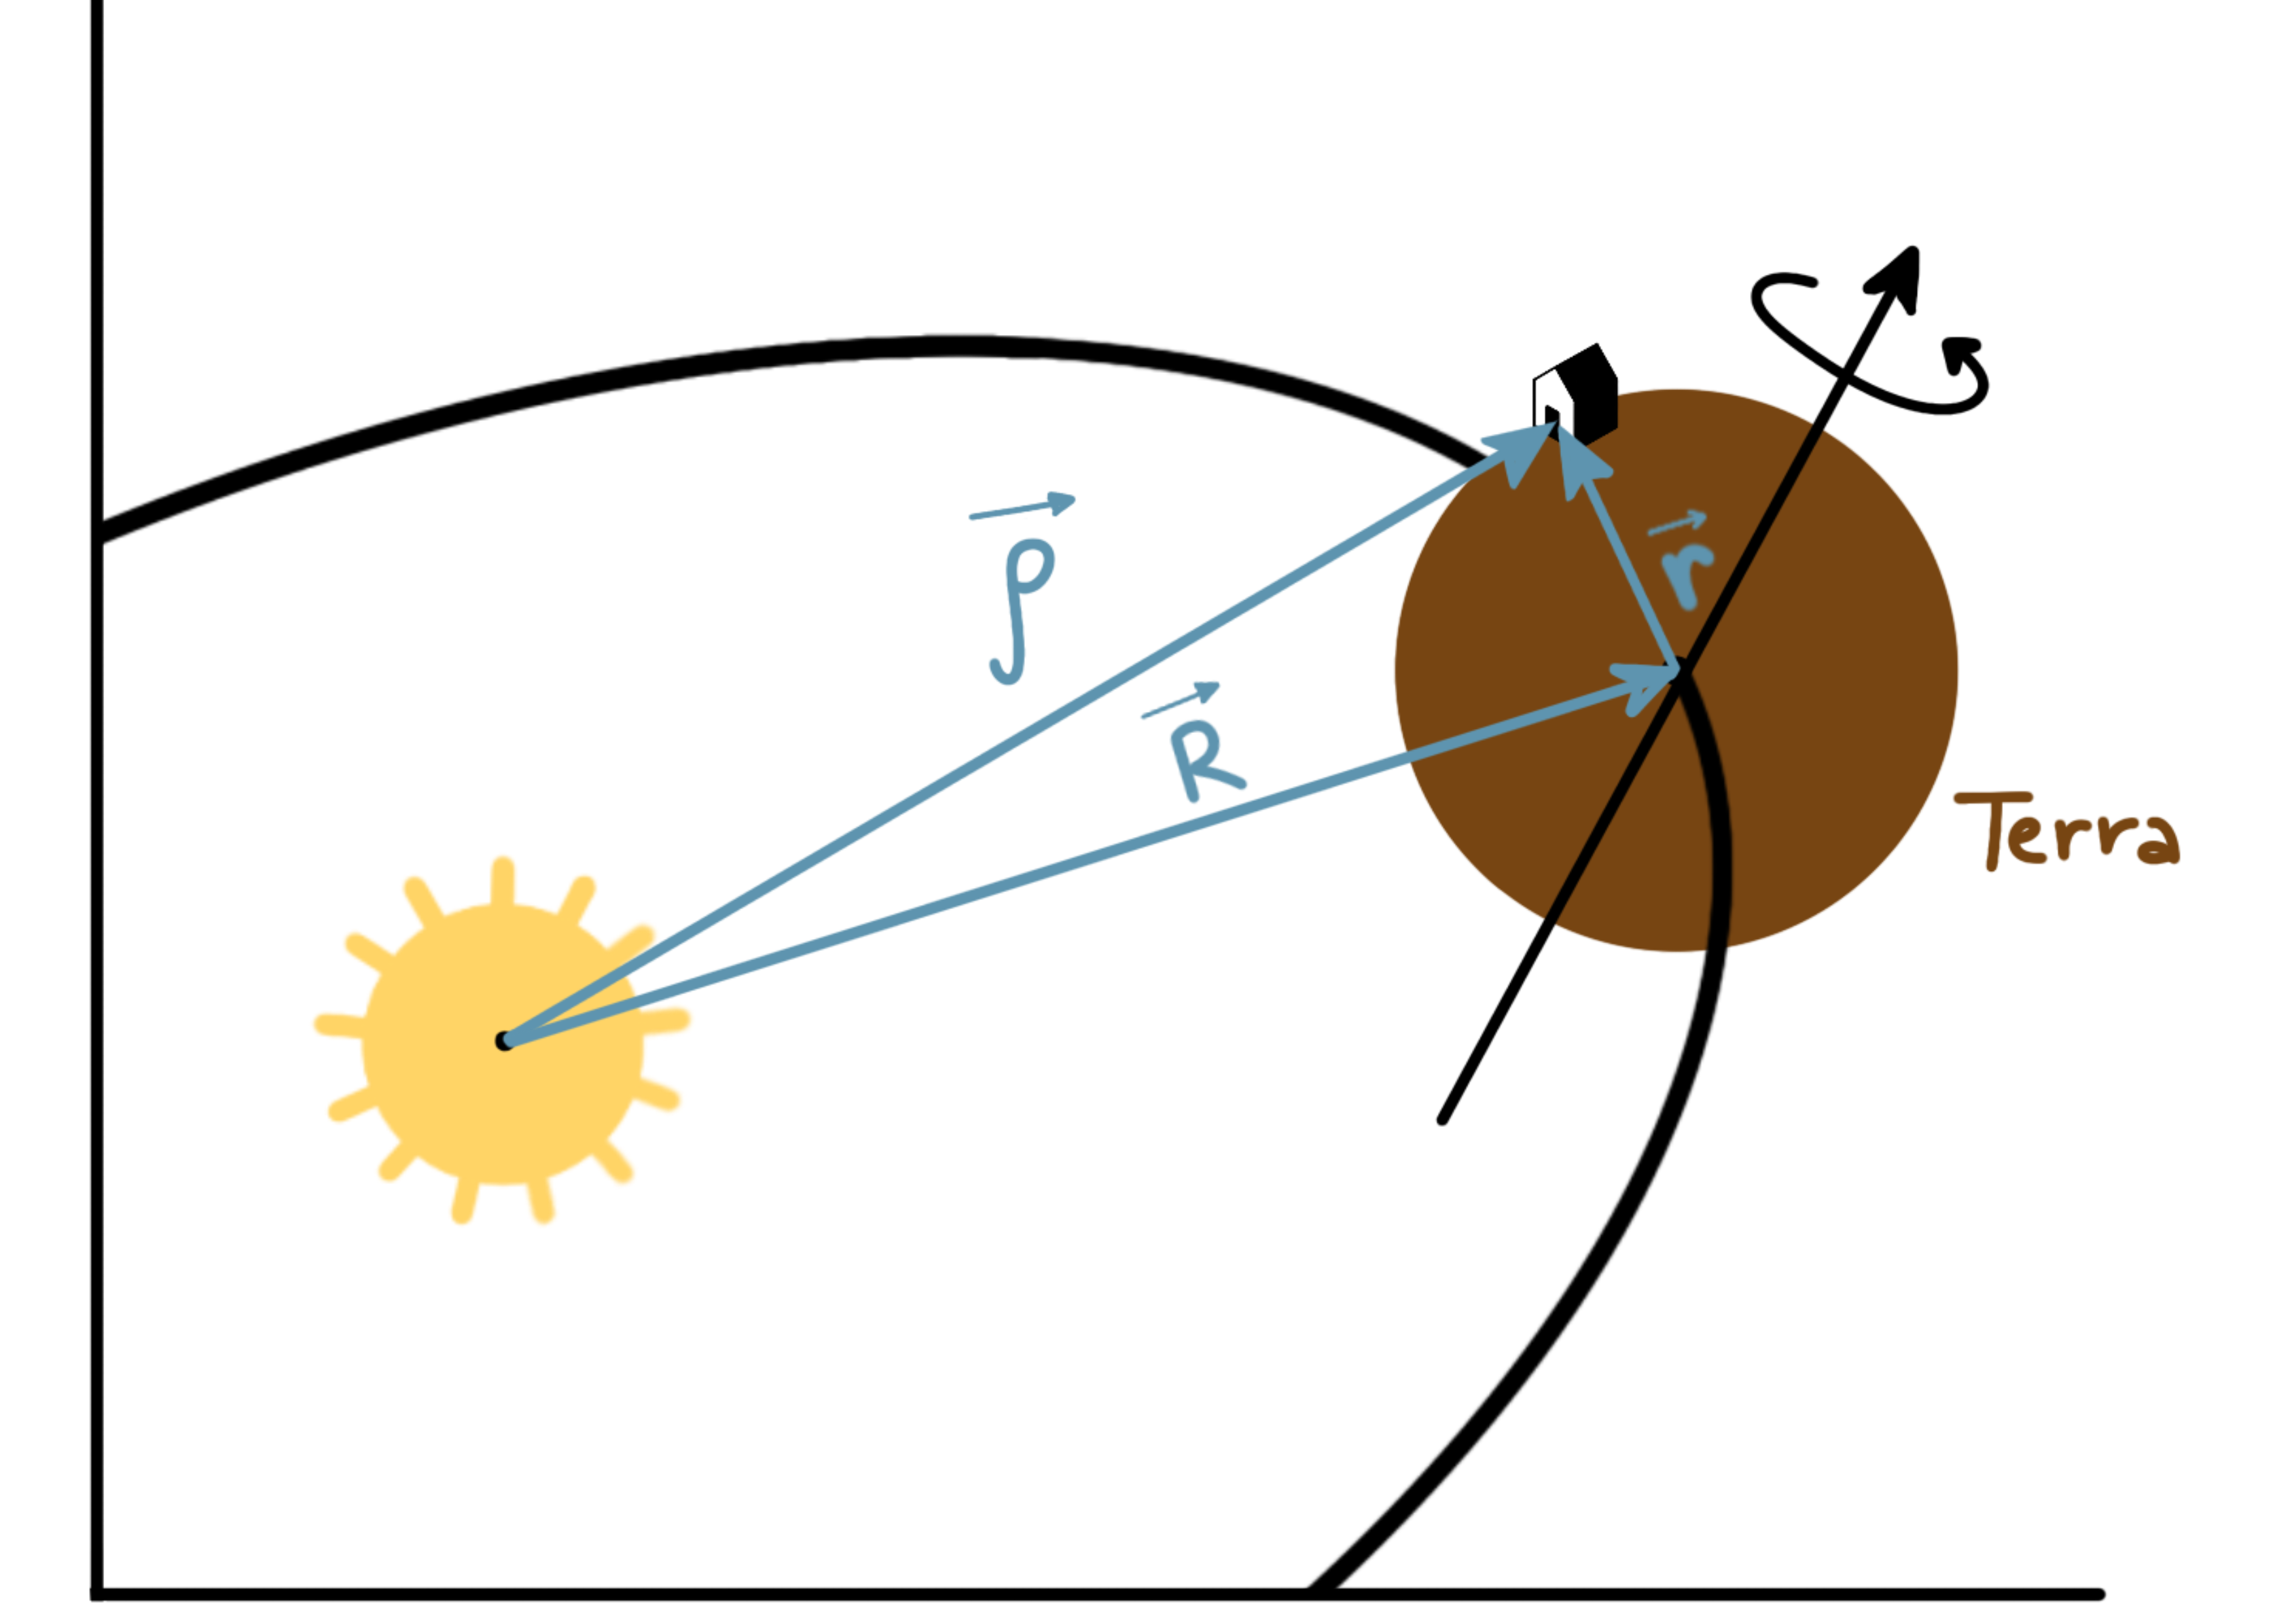
\includegraphics[width=\textwidth]{vectors.PNG}
        \caption{Els vectors que hem definit a la secció \ref{sec: seccio_2}.}
        \label{fig: sist_vectors}
    \end{subfigure}%
    \hspace{0.000001\textwidth}%
    \begin{subfigure}{0.5\textwidth}
        \centering
        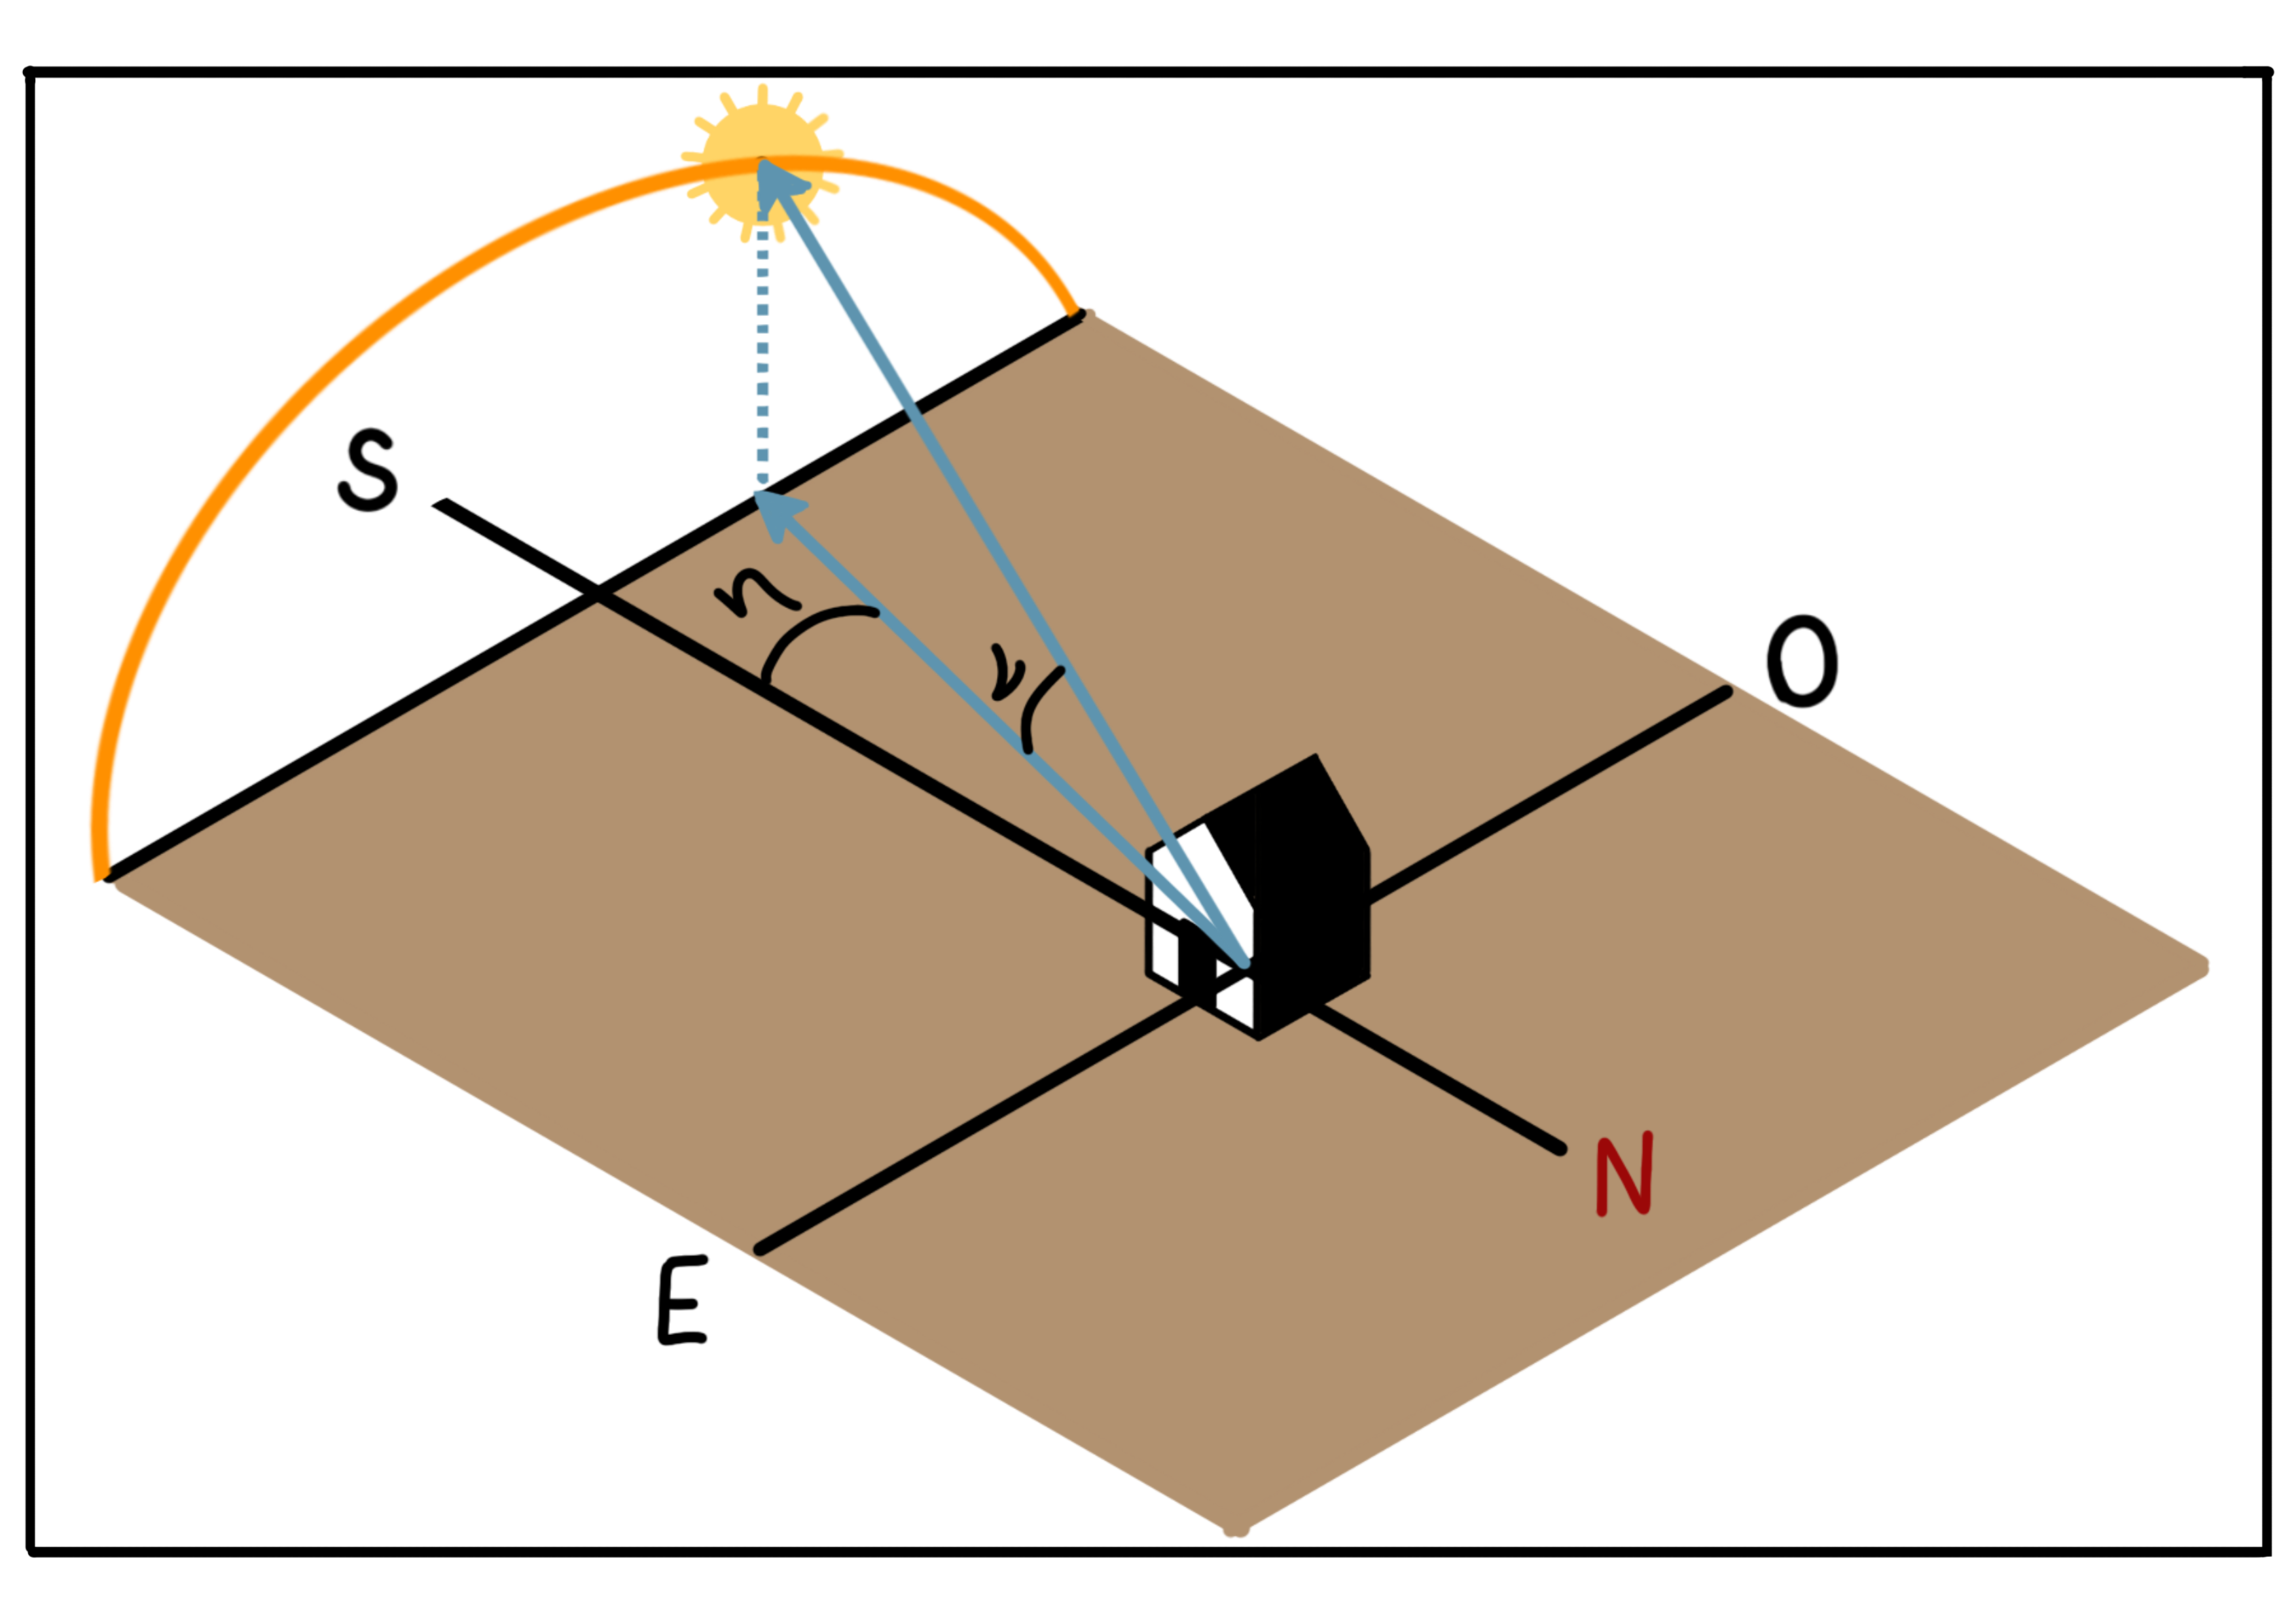
\includegraphics[width=\textwidth]{ang_sol.PNG}
        \caption{Els dos angles que hem usat per a determinar la posició del Sol.}
        \label{fig: sist_sol}
    \end{subfigure}
\end{figure}

\begin{figure}[hbt]
    \centering
    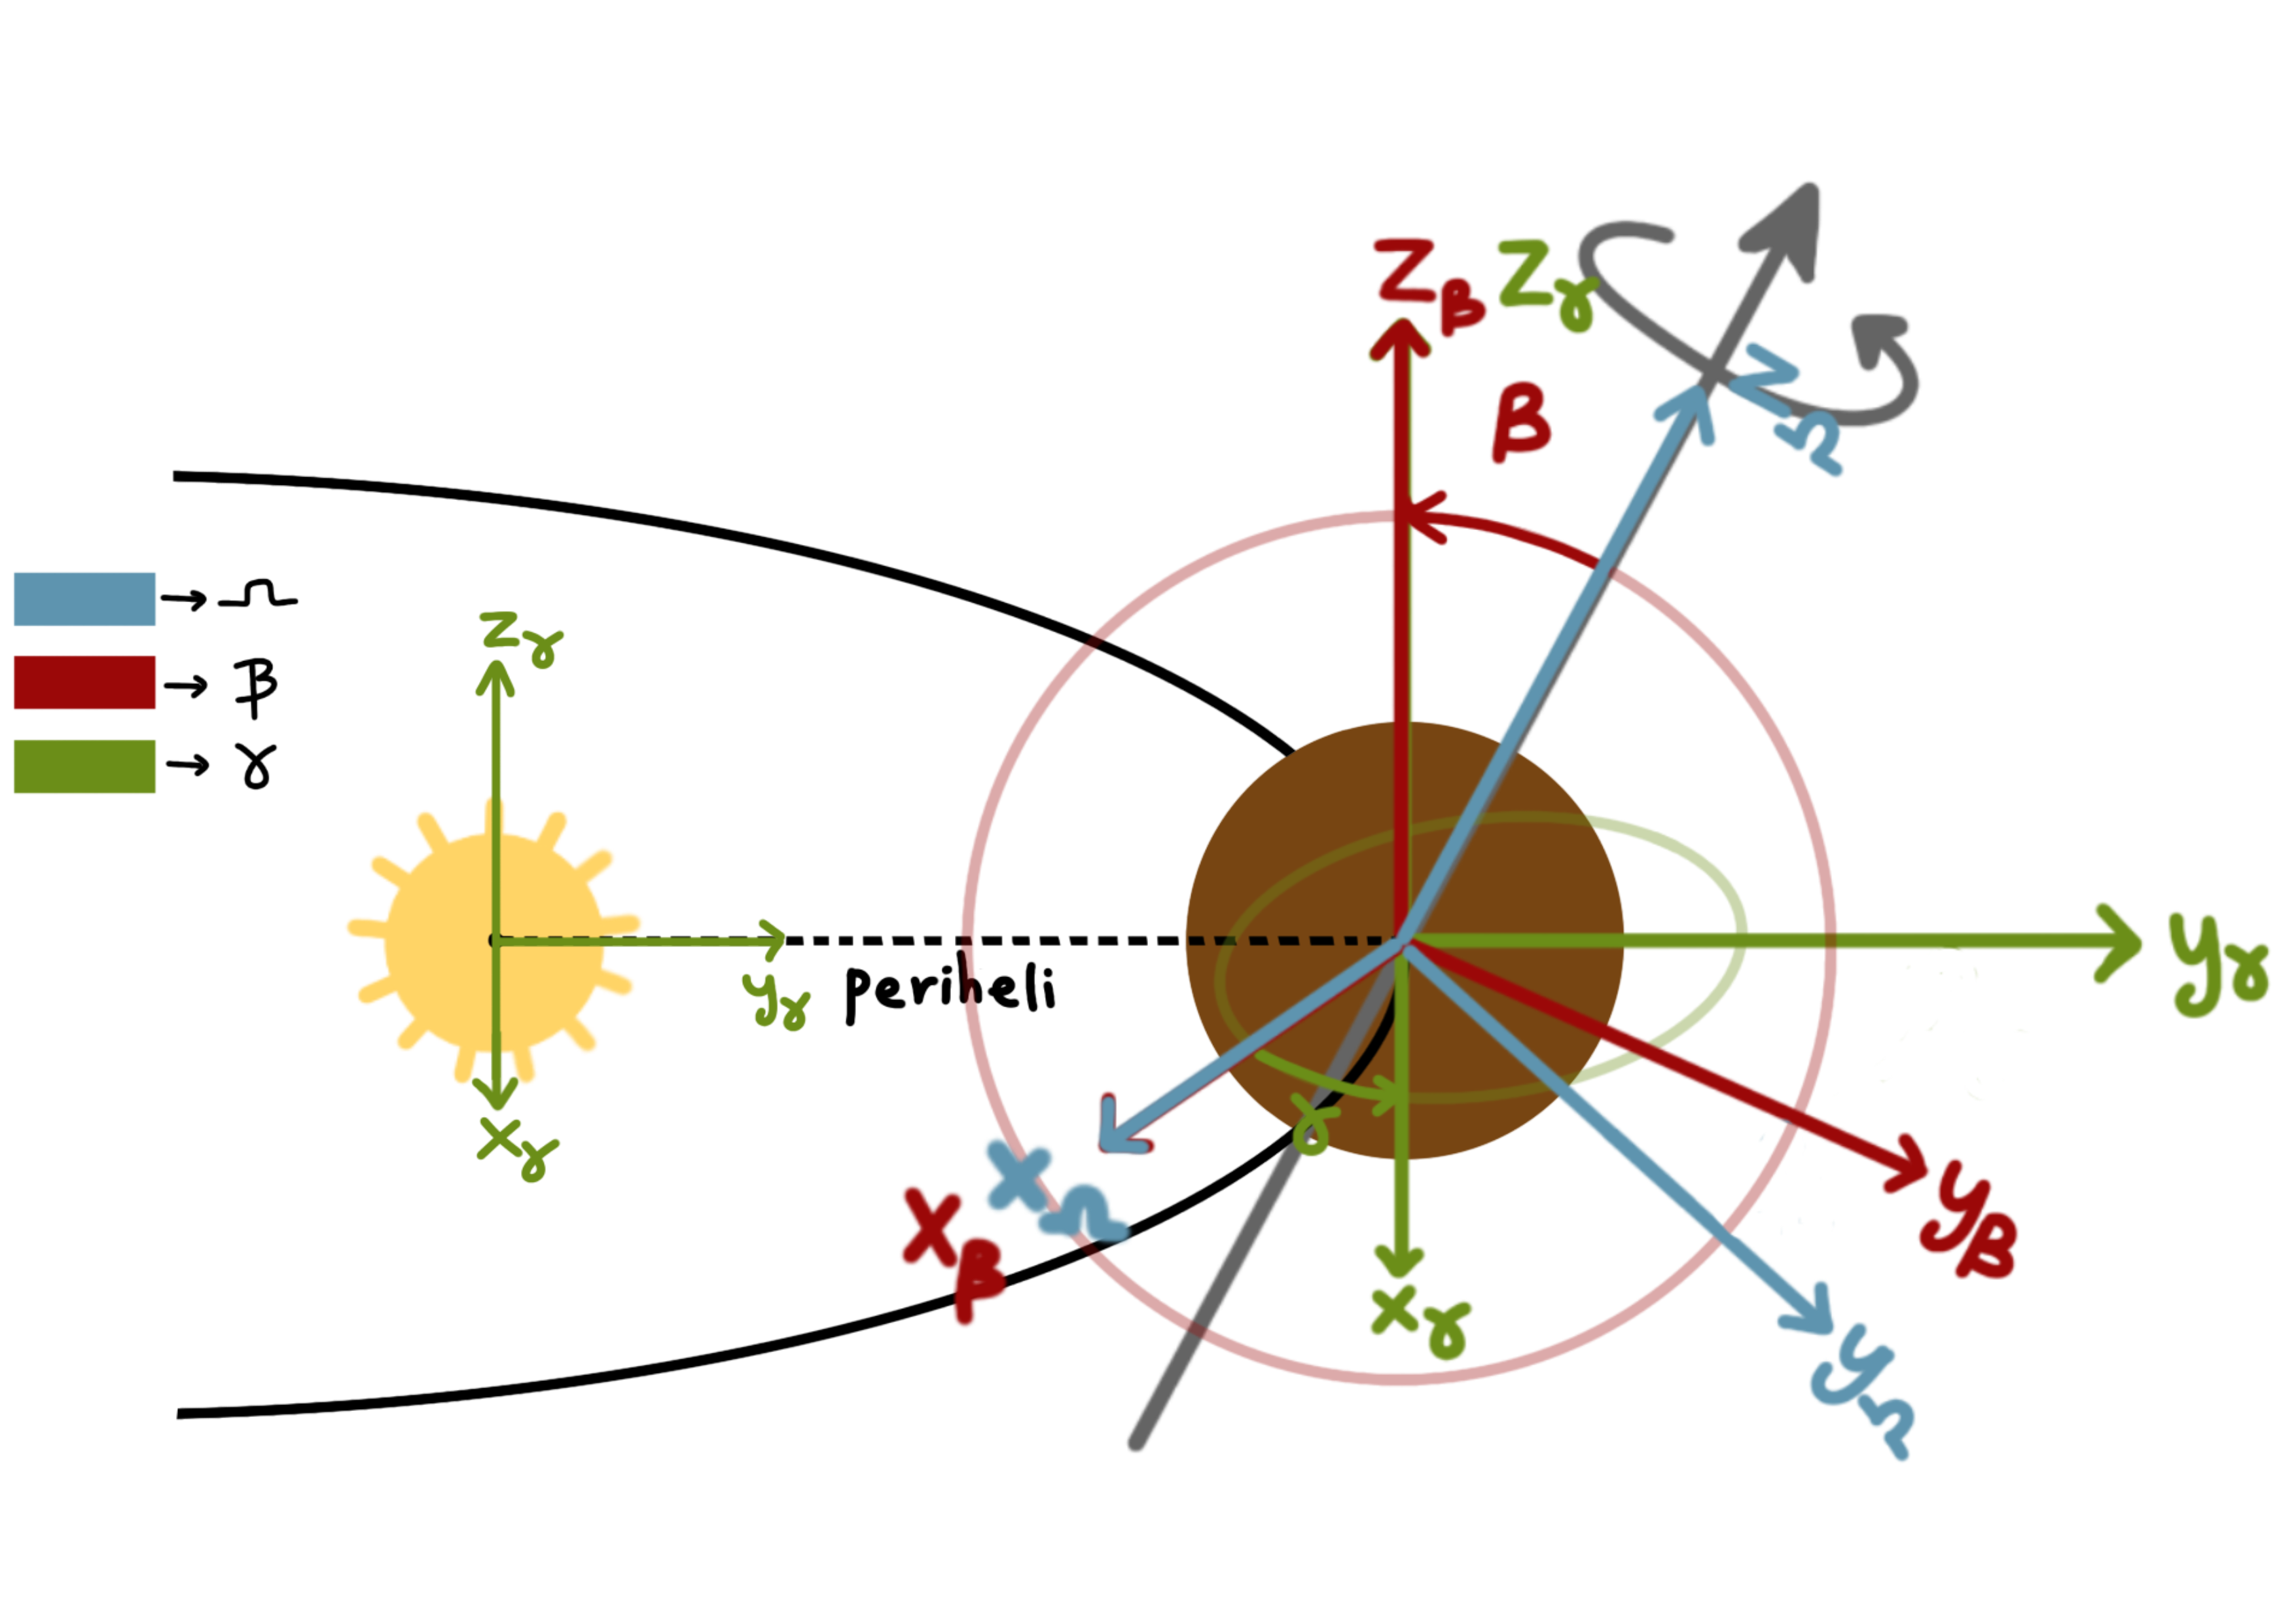
\includegraphics[width=0.5\textwidth]{sist_ref.PNG}
    \caption{Diferents sistemes de referència de la secció \ref{sec: seccio_2}.}
    \label{fig: sist_ref}
\end{figure}

\section{Valors numèrics}
\label{sec: valors numerics}
\section{Demostració de l'Eq. \eqref{cos theta}}
\label{sec: cos theta}
En aquest apartat demostrarem l'Eq. \eqref{cos theta}.

A continuació definim els angles que apareixen en l'equació.
\begin{itemize}
    \item $\beta$, \textbf{Angle zenital de la placa (inclinació)}: l'angle que formen el pla de la placa i l'horitzontal; $0^\circ \leq \beta \leq 180^\circ$.
    \item $\gamma$, \textbf{Angle azimutal de la placa}: la desviació de la projecció sobre un pla horitzontal de la normal a la superfície respecte el meridià local. Prenem com a $\gamma=0$ la direcció sud, i els valors negatius indiquen desviació cap a l'est i els positius cap a l'oest; $-180^\circ \leq \gamma \leq 180^\circ$.
    \item $\theta_z$, \textbf{Angle zenital solar}: l'angle entre la vertical i la radiació solar incident; $-180^\circ \leq \beta \leq 180^\circ$.
    \item $\gamma_s$, \textbf{Angle azimutal solar}: l'angle entre la projecció sobre un pla horitzontal de la direcció de la llum incident respecte el meridià local, seguint el mateix conveni de signes que per $\gamma$; $-180^\circ \leq \gamma \leq 180^\circ$.
\end{itemize}


\section{Discussió Núria potència}

En la Fig. \ref{fig: potencia dia 1} com més proper és el valor de $\gamma$ a 0$^{\circ}$, major és el valor màxim de la potència. D'altra banda, per un determinat $\gamma$, la menor potència màxima assolida és per $\beta=0^{\circ}$. En el cas del dia 170, representat a la Fig. \ref{fig: potencia dia 170}, la potència màxima quan $\beta=0^{\circ}$ és notablement superior a la del dia 1. D'altra banda, la gràfica per $\beta=35^{\circ}$ al migdia s'observa una disminució en la potència. A més, en tots els casos la duració de la generació de potència és superior a la del dia 1. Tot això es deu a que el dia 170 és d'estiu. Per tant, la posició del Sol és més alta de manera que quan està al voltant de la seva alçada màxima l’angle $\theta$ és major per $\beta=0^{\circ}$, i disminueix amb la inclinació de la placa.



\begin{figure}[H]
    \centering
    \begin{subfigure}{0.5\textwidth}
        \centering
        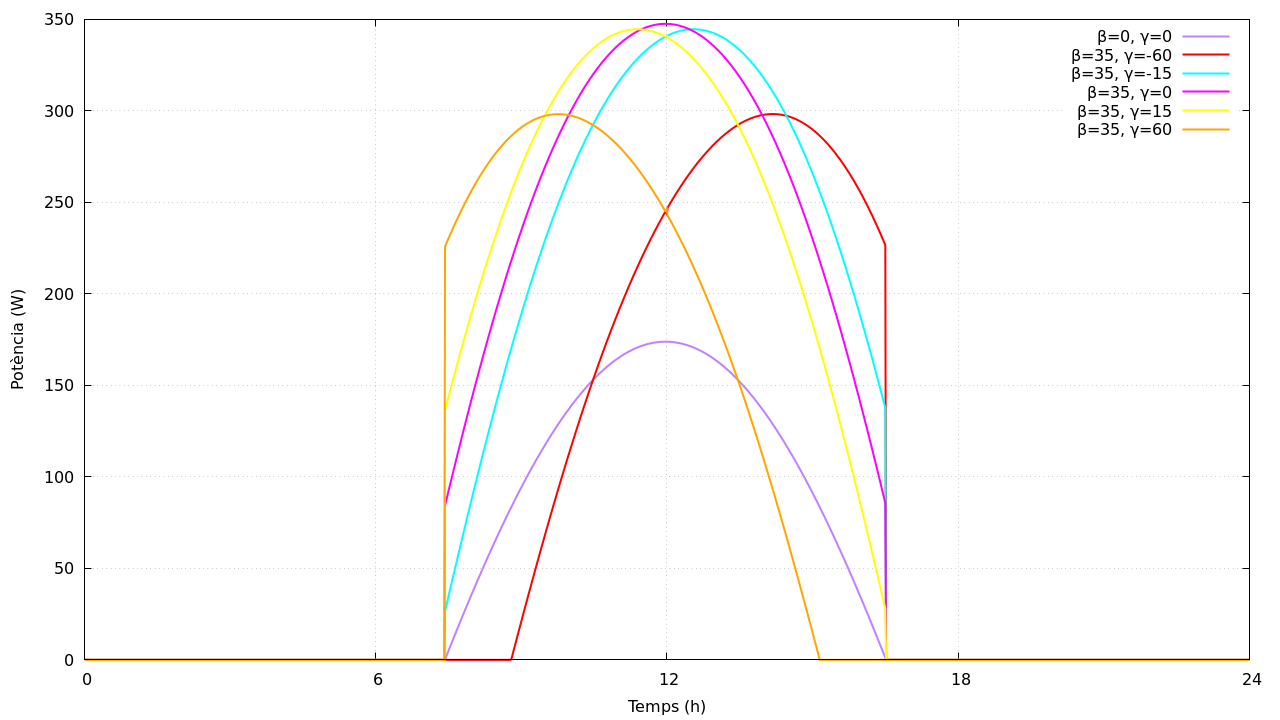
\includegraphics[width=\textwidth]{dia1_pot_plot.png}
        \caption{Dia 1.}
        \label{fig: potencia dia 1}
    \end{subfigure}%
    \hspace{0.000001\textwidth}%
    \begin{subfigure}{0.5\textwidth}
        \centering
        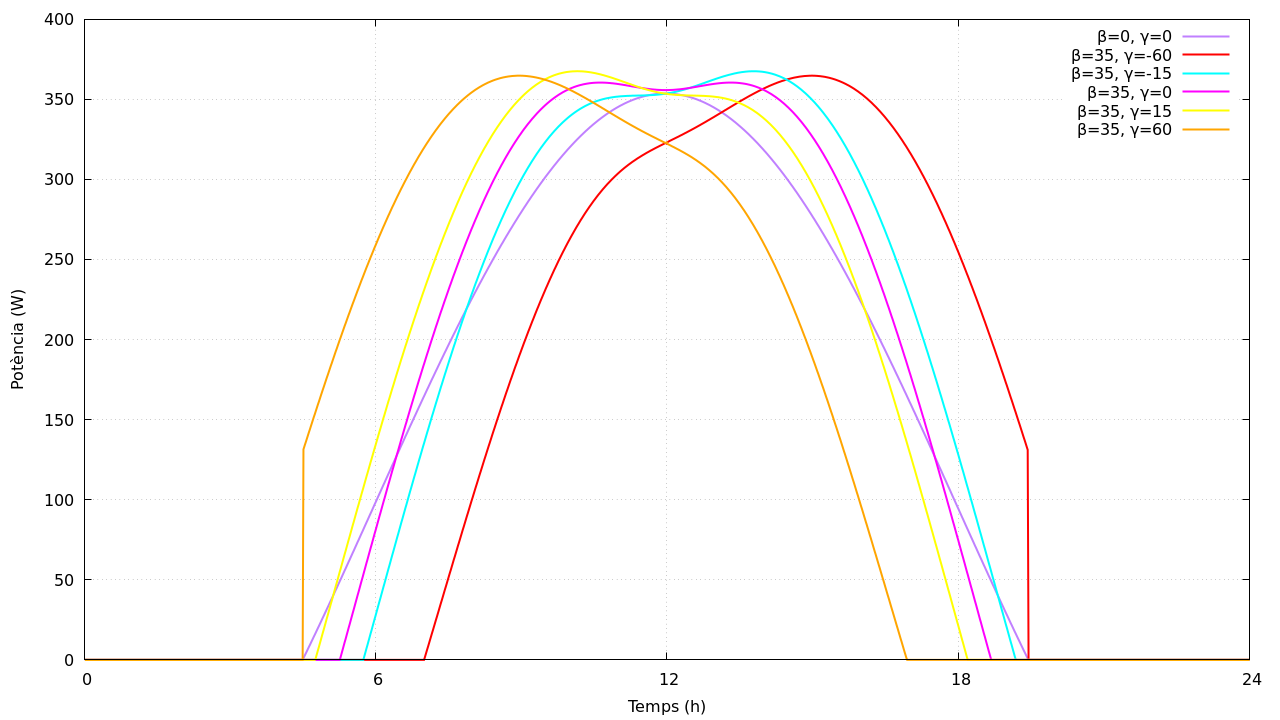
\includegraphics[width=\textwidth]{dia170_pot_plot.png}
        \caption{Dia 170.}
        \label{fig: potencia dia 170}
    \end{subfigure}
    \caption{Potència elèctrica produïda per la placa durant un dia per diversos valors de $\beta$ i de $\gamma$.}
    \label{potencia un dia}
\end{figure}


\end{document}
